\documentclass{report}
\usepackage[utf8]{inputenc}
\usepackage{times}
\usepackage{cite}
\usepackage{hyperref}
\usepackage{tablefootnote}
\usepackage{graphicx}
\usepackage{float}
\restylefloat{table}
\usepackage{listings}
\usepackage{xcolor}
\usepackage{enumitem}
\usepackage{array}
\usepackage{longtable}
\usepackage{multirow}
\usepackage{titlesec}

\setcounter{tocdepth}{5}
\setcounter{secnumdepth}{5}

\newcommand{\specialcell}[2][l]{%
  \begin{tabular}[#1]{@{}l@{}}#2\end{tabular}}


\titleformat{\paragraph}
{\normalfont\normalsize}{\theparagraph}{1em}{}
\titlespacing*{\paragraph}
{0pt}{3.25ex plus 1ex minus .2ex}{1.5ex plus .2ex}

% set the default code style
\lstset{
    frame=tb, % draw a frame at the top and bottom of the code block
    tabsize=4, % tab space width
    showstringspaces=false, % don't mark spaces in strings
    commentstyle=\color{green}, % comment color
    keywordstyle=\color{blue}, % keyword color
    stringstyle=\color{red}, % string color
    basicstyle=\footnotesize
}

\hypersetup{
    colorlinks,
    citecolor=black,
    filecolor=black,
    linkcolor=black,
    urlcolor=black
}



\title{Smartphone App Concept for Medical Applications.}
\author{Alexander Gustafson\\
  University of Applied Sciences,\\
  Zürich,\\
  Switzerland,\\
  alex\_gustafson@yahoo.de}
\date{\parbox{\linewidth}{\centering%
  \today\endgraf\bigskip
  Dozent: Reto Knaack (knaa@zhaw.ch)\endgraf\bigskip
  School of Engineering, Abteilung Zürich \endgraf
  Studiengang Informatik\endgraf
  }}





\begin{document}
\maketitle

\chapter*{Abstract}
The market for smartphone based medical applications is a relatively new and growing quickly. The majority of medical apps are relatively simple health management and tracking applications that might remind a user to take his or her medicine or monitor blood pressure and heart rate data provided by accompanying devices. However, more sophisticated apps can directly provide diagnostic information by capturing and analysing data directly. Several apps exist that can asses the risk of skin cancer by tracking changes in the growth of skin lesions over time.


\tableofcontents

\chapter{Introduction}
\section{Background}

Modern smart phones have opened new possibilities in all kinds of fields. For medical applications the combination of high resolution cameras, sensor devices, powerful CPUs and mobile networking capabilities could even be life saving. By combining input devices with powerful algorithms it should be possible to provide important diagnostic information that can inform it’s user of impeding risks. One particularly interesting medical application would be the detection of melanoma in a skin lesion using a mobile phone.

Melanoma is a type malignant skin tumour that develops from benign melanocytic nevi. Although less frequent than other skin cancer types, it causes more deaths \cite{cancer_gov_skin}, and it’s incidence is increasing dramatically, especially in the young white population \cite{S_ez_2013}. Early diagnosis and treatment is vital.

Several non-invasive techniques exist which dermatologist can employ to visually make a diagnosis. The most common are pattern analysis, the ABCD rule, the 7-point checklist and the Menzies method, among others \cite{marghoob2004atlas}. These methods generally use a combination of defined visual clues and indicators to assess the risk of a skin lesion. CAD ( Computer Aided Diagnosis ) systems exists that can assist a dermatologist, and even provide automatic diagnosis with an accuracy comparable to that of doctors trained in dermoscopic techniques \cite{Filho2015}.


\section{Project Description}

This bachelor project will investigate the following questions:

\noindent
\begin{itemize}
\item What smartphone based medical apps are available that can track and assess the risk of skin lesions?
\item What methods and algorithms can be employed by mobile phones to calculate the risk?
\item What is necessary to build a mobile app that can provide a risk assessment of skin cancer melanoma from captured images?

\end{itemize}

\section{Goals}

\noindent
\begin{enumerate}
\item Research the medical app market to gain an overview of areas of development, what apps are available, what trends are discernible. Of special interest are apps that use internal sensors ( e.g., camera ) and mathematical algorithms to detect skin cancer melanoma.

\item Gain familiarity with machine learning and image recognition algorithms. Describe the basic principles of these algorithms.
\item Research and compare available data and algorithms (e.g. in computer vision / machine learning). Define the relevant attributes that can be used to train the algorithm. This can also include changes in size over time.

\item Based on the research and comparison choose a specific algorithm and data with which to proceed. The algorithm must be able to
\begin{enumerate}
\item identify the skin lesion correctly,
\item compute the relevant attributes,
\item use these attributes to classify the skin lesions whether it is possibly cancerous or not
\end{enumerate}
\item Implement the algorithm as a prototype ( using Python for example ). Using images of a skin lesion as input, the algorithm will provide a risk assessment as output. Implement tests that can calculate the accuracy of the algorithm. Compare the implemented algorithm with at least one other algorithm.

\item Create a concept for a medical mobile app that can utilise the features of modern smartphones to provide a risk assessment of skin cancer melanoma based on captured images. This includes a full requirements analysis, i.e. use cases, functional / non-functional requirements, architecture.

\item Implement as proof of concept specific aspects of the medical mobile app.

\end{enumerate}

\section{Expected Results}

\noindent
\begin{enumerate}
\item Results of the medical app market research including graphical presentation of trends and statistics.
\item Documentation of the available data and algorithms including high level excursion into the theory behind machine learning and image recognition algorithms.
\item Comparison of available data and algorithms. Definition of relevant attributes.
\item Decision, which algorithm to use.
\item Documentation of the implementation of the algorithm, including tests, evaluation and comparison with at least one other algorithm.
\item Documentation of a concept for a medial app, including defined use cases, requirements, architecture and implemented design patterns.
\item Proof of Concept: implementation of specific aspects of the medical mobile app.
\end{enumerate}

\chapter{Market Research}


\section{Data Gathering}

\subsection{Gathering Data from the Apple iTunes Store}

Searching the Apple iTunes store is typically done manually via the iTunes Application from which text and data cannot be automatically extracted. Therefore, searching for and gathering data about IOS Applications is not easy. However, Apple does provide an rss feed that can be used to list Apps in specific categories and ordered according to how new, or how popular they are and if they are free or not. The rss feed is limited to 100 items per category. The data provided by the rss feed is minimal, not much more than title and a text description of the app. There are no sub-genres or tags than can be used to further differentiate the apps.

Using a python script data was gathered from the following rss feeds:

Top 100 Free Medical Apps
Top 100 Grossing Medical Apps
Top 100 Paid Medical Apps
This combined results included data about 255 IOS apps. The title and description fields were imported into a database. Other information from the data such as price, right, or image link were ignored.


\subsection{Gathering App Data from the Google Play Store}

In order to gather data from the Goole app store a script was programmed that could extract lists of apps from a specific url. The following urls were scanned:
\noindent
\begin{itemize}
\item Top Paid Medical Apps : https://play.google.com/store/apps/category/MEDICAL/collection/topselling\_paid

\item Top Free Medical Apps : https://play.google.com/store/apps/category/MEDICAL/collection/topselling\_free
\end{itemize}

For each app listed the script would extract the url of the app's detail page. From the detail page more imformation would be gathered and stored in a database. The data set is similar to that of the itunes rss feed. The title and description text were imported, other fields such as pricing and copyright were ignored.

Data on 480 Medical Apps for Android was imported. However a significant percentage of the apps could not be classified because the description text was in a language other than English, German, or French.


\section{Categorization}

The term "Medical App" is broad and neither the iTunes nor Google app stores offer any kind of sub categorization. In order to get a better overview of what sort of Medical Apps are available it was necessary to manually browse the gathered data and assign categories to the apps.

A database management tool was created using the python based Django Web Framework. Django provides many tools that makes constructing and interacting with databases very easy. The built-in backend administration tool can be configured to browse, edit, and filter data.

In order to quickly browse through and categorize over 700 apps. The Django backend admin was configured so apps could be categorized one after the other with a minimum of clicks or scrolling. The user was presented a list of uncategorized apps. The first one is clicked. The user is then presented with a page displaying the title and summary text of the app and a field from which a category can be selected. Once saved, the app is no longer presented on the list, the user can select the next app at the top of the list.

\subsection{Description of Categories}
\noindent
\begin{itemize}
\item \textbf{Community} - provides some soft of social networking service through which the user can share data with her family or with a network of people suffering from similar disorders.
\item \textbf{Fun / Entertainment} - These apps have to real medical purpose. They are for enjoyment only.
\item \textbf{Alert / First Response} - Apps that assist first responders or that help users alert first responders that help is needed.
\item \textbf{Health / Lifestyle} - Relaxation and meditation apps, or ovulation and fertility reminders
\item \textbf{Resource Finder} - Apps that locate resources in the vicinitly, nearby pharmacies or care providers.
\item \textbf{Reminder} - Apps with timer or calendar functionality that might remind a user of an appointment or manage medince consumption.
\item \textbf{Algorithmic / Diagnostic} - These are apps that provide some sort of diagnositc information based on data that as been gathered by sensors or entered by the user. Examples are seizure detection apps, or stroke severity evalutaion apps.
\item \textbf{Learning / Educational / Reference} - By far the largest category, this includes apps that provide reference information about diseases or education material like anatomy apps for example.
\item \textbf{Organisational} - Apps in this category might help a user or practitioner organise, share or track data and documents. Examples are apps that help users track the status of their blood pressure or blood sugar levels, create health diaries, or manage clinical data and images.
\end{itemize}

\section{Results}


\subsection{IOS Medical Apps}

\begin{figure}[H]
    \centering
    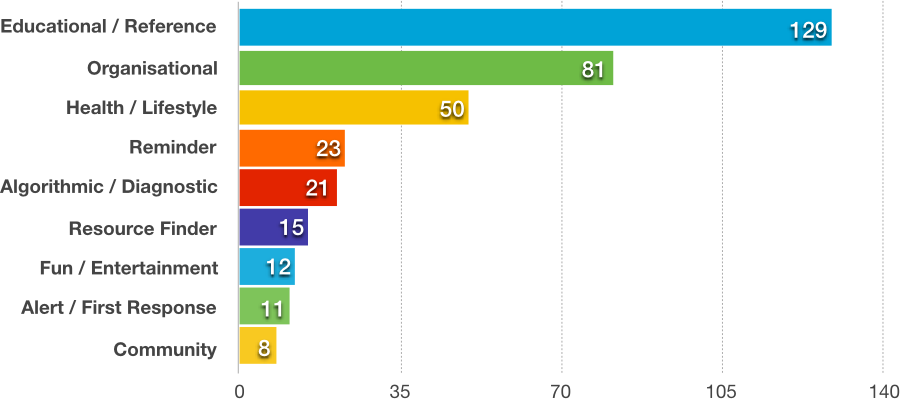
\includegraphics[width=\textwidth]{assets/market_research/apple_chart1.png}
    \caption{Medical Apps on the iTunes Apple Store, Search conducted on 17.05.2016}
    \label{fig:itunes_apps}
\end{figure}


\subsection{Android Medical Apps}

\begin{figure}[H]
    \centering
    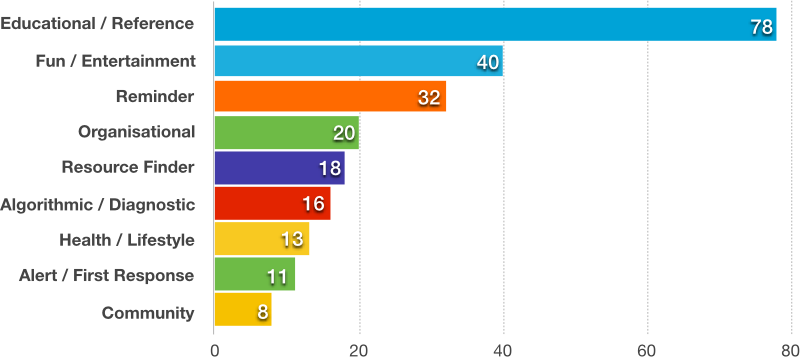
\includegraphics[width=\textwidth]{assets/market_research/android_chart.png}
    \caption{Medical Apps on the Goolge Play Store, Search conducted on 17.05.2016}
    \label{fig:android_apps}
\end{figure}

\subsection{Dermatology Apps 2013 vs 2016}

Mobile apps are an especially good fit for dermatology-related care. Most dermatological conditions are by nature visible. The initial diagnosis and follow up monitoring is mostly done visually. A mobile device with a camera can aid patients and practitioners in the diagnosis of a dermatological condition and tracking it's development. The article Mobile Applications in Dermatology\cite{Brewer_2013} in 2013 identified 229 dermatology-related apps across 5 app platforms ( Android, Apple, Blackberry, Nokia, and Windows ). These were grouped into categories based on their primary functionality. The "Self-surveillance/diagnosis" category was the second largest on the Android and Apple platforms, with 13 and 24 apps respectively.

\begin{figure}[H]
    \centering
    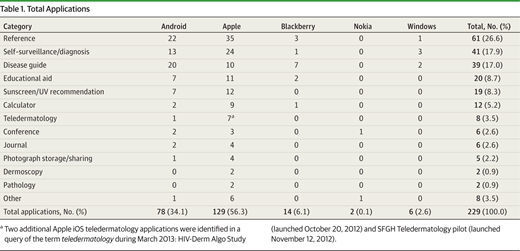
\includegraphics[width=\textwidth]{assets/market_research/brewer.png}
    \caption{Total Applications, Brewer 2013}
    \label{fig:brewer}
\end{figure}

Using the same search criteria and categories from the article above indicates that the availability of dermatological apps is growing. Today there are 33 dermatological apps on the Apple platform that can be identified as having "Self-surveillance/diagnostic" features. With the exception of the "Reference" category, all other categories show significantly higher numbers of available apps.


\begin{figure}[H]
    \centering
    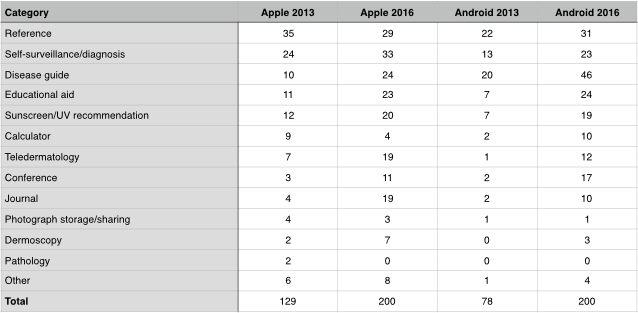
\includegraphics[width=\textwidth]{assets/market_research/apple2013vs2016.png}
    \caption{Demotological Apps by Category, July 2013(Brewer 2013) vs May 2016}
    \label{fig:apps_vs}
\end{figure}

It is important to note that the categories listed above are not defined in the stores. The apps must be manually assigned to a category based on an interpretation of the description text in the store and information obtainable on related websites. It is possible therefore that apps that were originally designated to the “Reference” category might have been interpreted in this paper as a “Educational aid” app for example. The interpretation of the functionality of an app is fuzzy in many cases, and many apps have some crossover functionality. An app developed for self-surveillance will often contain information pertaining to symptoms and treatment ( reference ).

\subsection{Dermatological Apps with Automatic Risk Assesment}

Of the 55 apps identified belonging to the "Self-surveillance/diagnosis" category, only 2 provided risk assesment features based on automatic analysis of captured images.

\noindent
\begin{itemize}
\item SkinVision : https://skinvision.com
\item mSkin Doctor
https://play.google.com/store/apps/details?id=com.maleemtaufiq.mSkinDoctor
\end{itemize}


\chapter{Image Data Sources}
\section{Dermofit}

High quality clinical images with corresponding masks. Great for training and testing.

\begin{table}[H]
\small
    \begin{tabular}{ | l | p{3.5cm} | l | p{3.5cm} |}
    \hline
    Image Type &  Description & Amount & Comment\\ \hline
    Actinic Keratosis &  Pre-cancerous patches of flakey or crusty skin, can develop into Squamous Cell Carcinoma
        & 45 & Not useful as comparison against melanoma \\ \hline
    Basal Cell Carcinoma &  Abnormal, uncontrolled growths of the skin's basal cells.
        & 239 & Not useful as comparison against melanoma \\ \hline
    Dermatofibroma &  Common and benign skin tumour.
        & 65 & Useful as comparison, some extreme cases might have to be left out of the training set. \\ \hline
    Haemangioma &  A collection of small blood vessels that form a lump under the skin.
        & 97 & Useful as comparison, some extreme cases might have to be left out of the training set \\ \hline
    Intraepithelial Carcinoma &  A type of squamous cell skin cancer limited to the upper layer of the skin.
        & 97 & Not useful \\ \hline
    Malignant Melanoma &  A type of cancer that develops from the pigment-containing cells known as melanocytes.
        & 76 & This is our baseline set, half will be used for training, the other half for testing \\ \hline
    Melanocytic Nevus &  Typical mole, benign.
        & 331 & Very usefull as comparison to Melanoma \\ \hline
    Pyogenic Granuloma &  Common skin growth, small, round and red in color due to large number of blood vessels.
        & 24 & Not usefull \\ \hline
    Seborrhoeic Keratosis &  Common non-cancerous skin growth.
        & 257 & Maybe usefull \\ \hline
    Squamous Cell Carcinoma &  Abnormal and uncontrolled growth of squamous cells in the epidermis.
        & 88 & Not usefull \\ \hline

    \end{tabular}

    \caption{Dermofit Image Categories}
    \label{fig:derm_cat}

\end{table}

\section{DermQuest}

Online teaching and learning resource with large image database.

Image were selected based on their usefullness for this project. Usefullness is based on quality and type of image. Dermoscopic images were not selected. Instead images were taken that appeared to be taken with a standard camera. The images only contained the mole to be examined and the surrounding skin area. No other details like eyelids, ears, or dark shadows.

Subgroups of Melanocytic Nevus were chosen. Dysplastic and Intradermal Nevus for the non-cancerous cases, and Malignant Melanoma as the cancerous cases.

\begin{table}[H]
\small
    \begin{tabular}{ | l | p{3.5cm} | l | p{3.5cm} |}
    \hline
    Image Type &  Description & Amount & Comment\\ \hline
    Benign Keratosis &
        & 5 &  \\ \hline
    Malignant Melanoma & A type of cancer that develops from the pigment-containing cells known as melanocytes.
        & 39 & This is our baseline set, half will be used for training, the other half for testing \\ \hline
    Melanocytic Nevus & Typical mole, benign.
        & 51 & Very usefull as comparison to Melanoma \\ \hline

    \end{tabular}

    \caption{DermQuest Image Categories}
    \label{fig:dquest_cat}

\end{table}

\section{PH2Dataset}

Demascopic Images

Many of the mole images extend almost to or even beyond the image border. This makes some of the processing difficult. However the images include an excel spreadsheet which clearly designates what type of mole, including some scoring info such as Asymmetry and Color information.
Includes border mask images.

\begin{table}[H]
\small
    \begin{tabular}{ | l | p{3.5cm} | l | p{3.5cm} |}
    \hline
    Image Type &  Description & Amount & Comment\\ \hline
    Common Nevus &
        & 79 &  \\ \hline
    Atypical Nevus &
        & 79 &  \\ \hline
    Melanoma &
        & 39 & Baseline set for training \\ \hline

    \end{tabular}

    \caption{PH2 Image Categories}
    \label{fig:ph2_cat}

\end{table}

\chapter{Image Feature Extraction}
A digital image is a matrix of pixels that contain color information, typically comprised of the 3 color channels red, green, and blue. A person can look at an image and quickly make statements about it's content. For instance, someone might look at an image of a street scene and be able to easily say "This is an image of a street in a town, there is one automobile, three people and a building in this scene". A person would easily be able to draw outlines around the objects and be able to differentiate between areas in each object.

For a computer to be able to "make statements" about the contents of an image it must use algorithms to group together and differentiate between objects in an image. The grouping together and differentiating of areas in an image is known as \textit{segmentation}. The statements that a computer can make about the content of an image are usually of statistical nature and are refered to as \textit{feature extraction}. Before segmentation an image is goes through a \textit{preprocessing} stage in order to remove or reduce irrelevant information or noise.

There are no universal algorithms for preprocessing, segmentation, or feature extraction. The algorithms employed depend on the context of the images to be analyed and the type of information that one is looking for.


\section{Preprocessing}

When capturing an image using a dermatoscope the skin is illuminated equally over the skin area to be photographed. The dermatoscope captures hi-resolution images with low levels of noise. The amount of preprocessing required is limited to colour enhancement to achieve better segmentation results. Using a digital camera like those found in smartphones requires introduces other challenges \cite{auto_seg}.

Unequal illumination or shadows in the image can make it more difficult for the segmentation algorithm to precisely recognise the lesions border. Glare from too much illumination, noise introduced by the circuitry of the sensor in the digital camera or hairs on the skin can also make it difficult to differentiate between the lesion area and healthy skin.

The preprocessing stage attempts to reduce the interference cause by these factors.


\subsection{Equalization}

Histogram Equalisation in image processing is the attempt to enhance detail in images that do not utilise the full range of pixel values. Important details in an image might not be clearly visible because they are is dark areas with low contrast. A histogram of the image is calculated. The histogram shows the distribution of pixels with respect to their brightness or intensity. The intensity of the pixels can be rescaled in order to be evenly distributed.

Depending on the content of an image though global histogram equalisation often makes dark areas darker, light areas become “washed out” and noise becomes more prevalent. This the opposite of what we would like to achieve for dermatological applications. Ideally the healthy skin would be a homogeneous colour and intensity, with no noise or disturbances except for the lesion area to be extracted.

Contrast Limited Adaptive Histogram Equalisation (CLAHE) is an adaptation of Histogram Equalisation but it is not global and it limits the contrast range. CLAHE analyses small regions, or tiles, of the image and enhances the contrast so that the local histogram matches a histogram specified a “Slope” parameter. The tiles are then interpolated together to prevent edge artifacts.

Figures \ref{fig:eq_A} to \ref{fig:eq_C} below show 3 examples of equalised images, comparing the global histogram  equalisation to the CLAHE method.

\begin{figure}[H]
    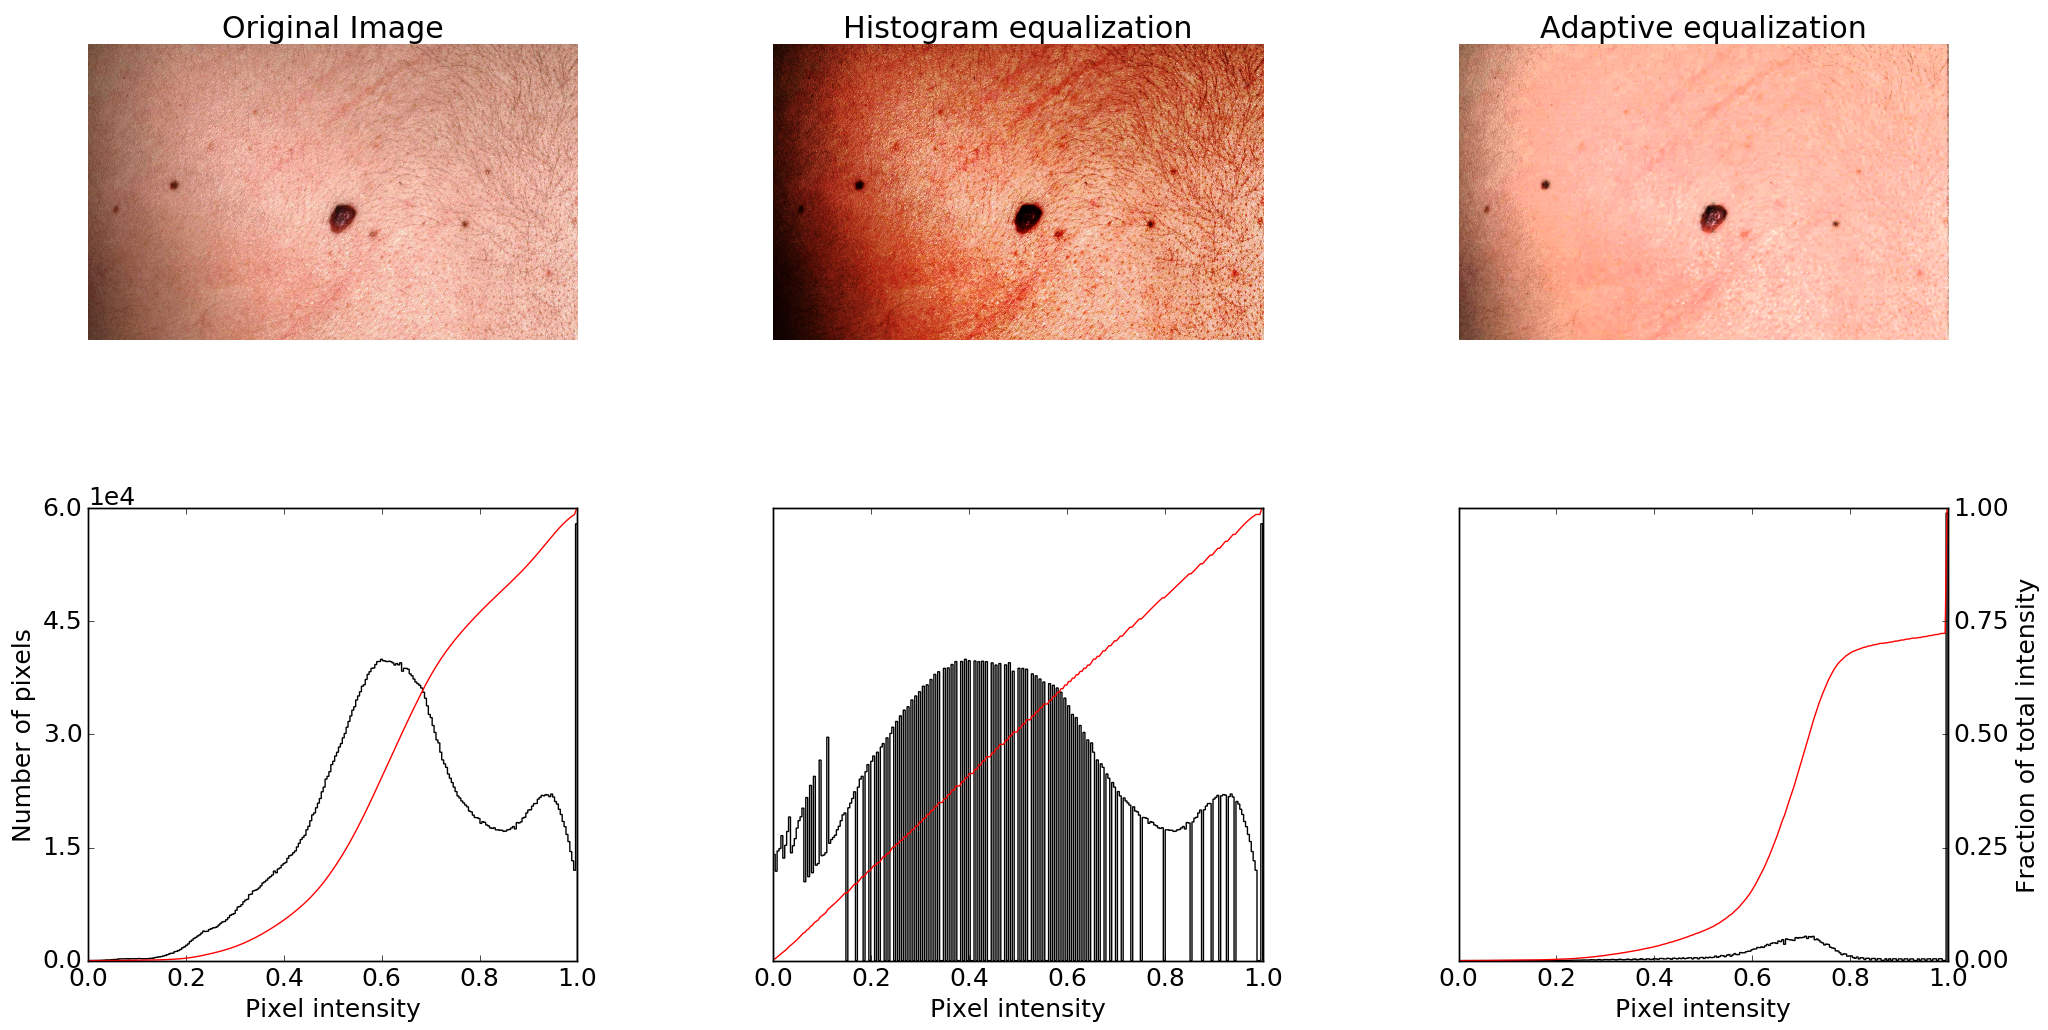
\includegraphics[width=\textwidth,keepaspectratio]{assets/image_processing/equalization/figure_01.png}
    \caption{Image Equalization Example A}
    \label{fig:eq_A}
\end{figure}
\begin{figure}[H]
    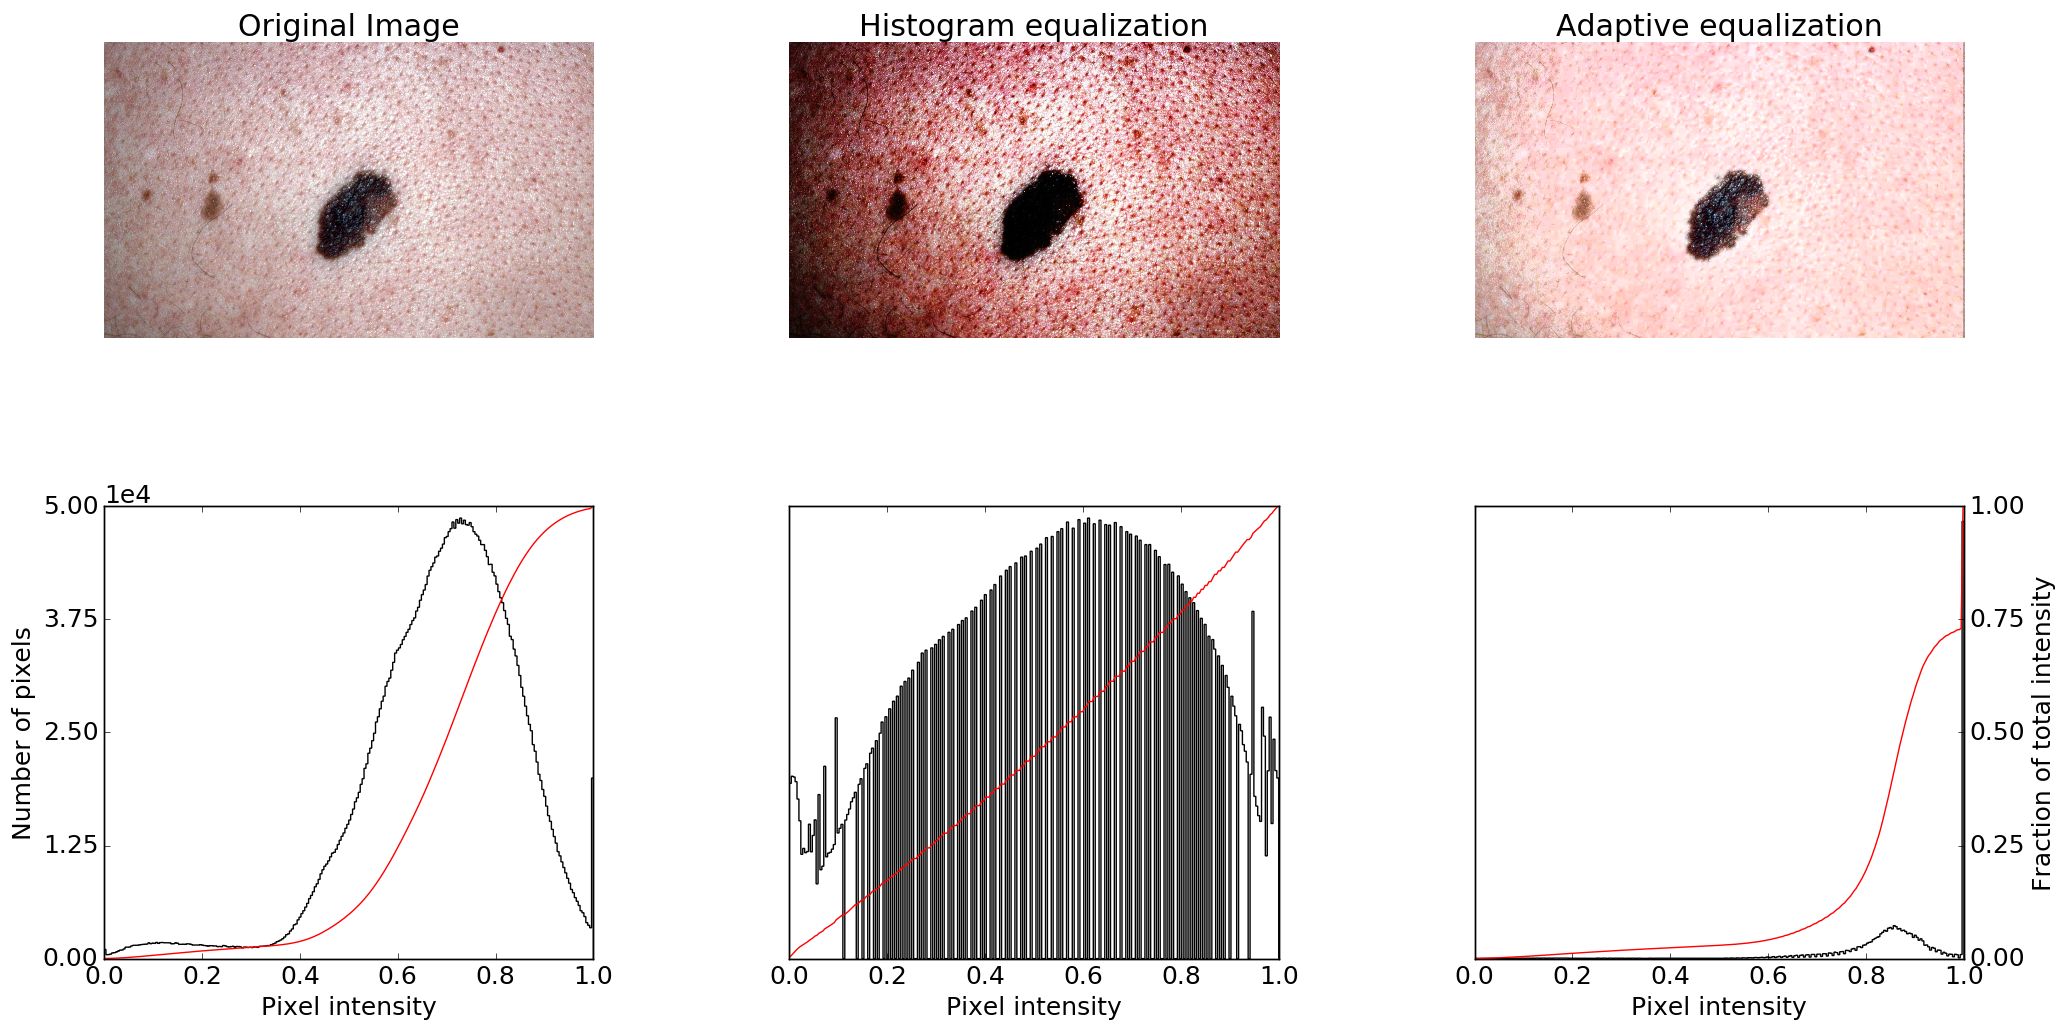
\includegraphics[width=\textwidth,keepaspectratio]{assets/image_processing/equalization/figure_02.png}
    \caption{Image Equalization Example B}
    \label{fig:eq_B}
\end{figure}
\begin{figure}[H]
    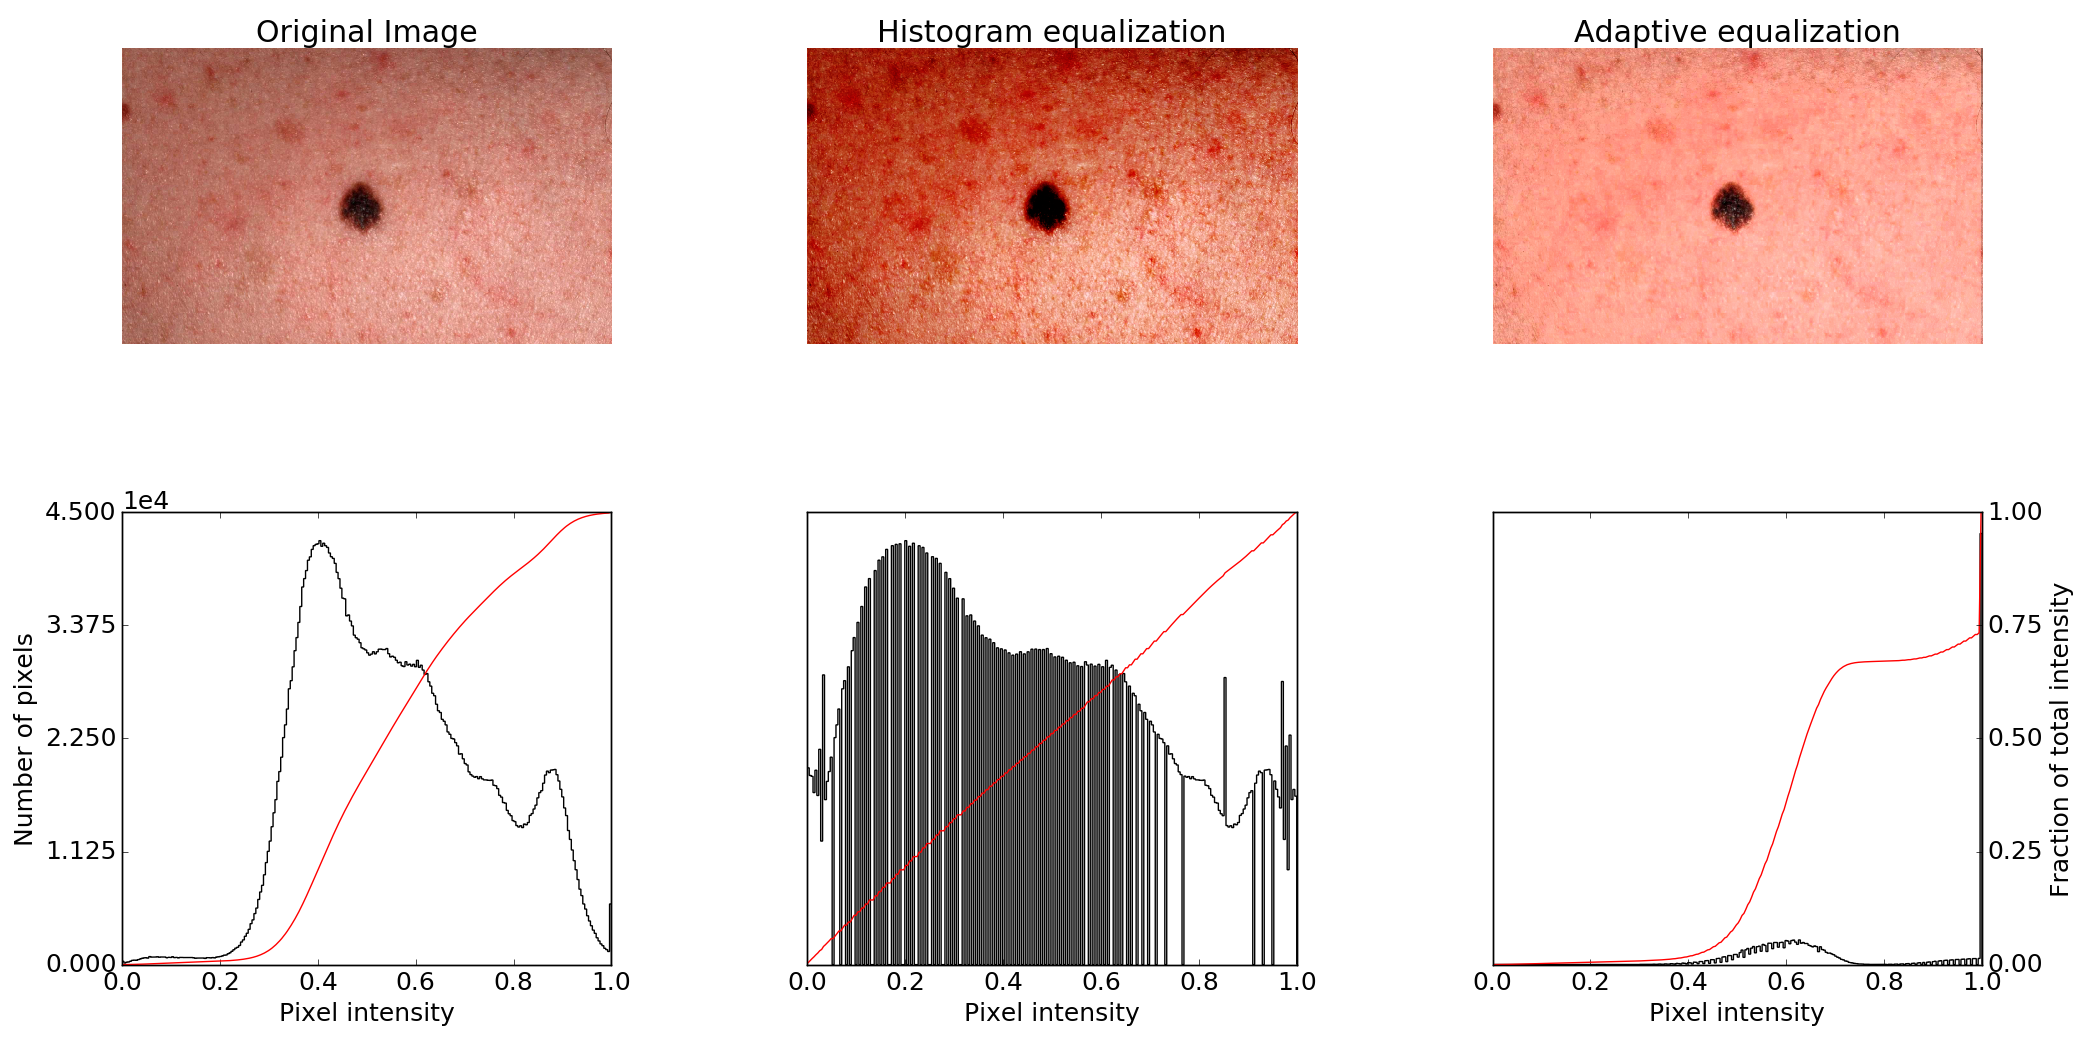
\includegraphics[width=\textwidth,keepaspectratio]{assets/image_processing/equalization/figure_03.png}
    \caption{Image Equalization Example C}
    \label{fig:eq_C}
\end{figure}

\subsection{Noise Reduction}

Noise in a captured image is inevitable, it will be introduced by the circuitry of the camera sensor or even from statistical quantum fluctuations of the photons known as “shot noise” \cite{image_noise}.  Noise in the image produces outlier pixels, pixels that do not represent the surface of the object in the image, and whose values diverge from neighbouring pixels.

Noise in the image will make it more difficult for the segmentation algorithms to achieve good accurate. Other challenges though might be reflectivity of the skin’s surface, the texture of the skin, or surrounding or intersecting the skin lesion.

Typical noise reduction techniques will analyse sections (often referred to as “windows” or “tiles”) or the image at a time and employ some sort of averaging function to the pixel values. The gaussian and median filters are common noise reduction functions.

\subsubsection{Gaussian Filter}

The Gaussian Filter is a low pass filter that reduces high frequency components of an image. It's main parameter is sigma which defines the width or distribution or the gaussian function. Higher sigma values cause pixels to be averaged with more of their neighbours. The visual result is a blurring of the image. The Gaussian Filter is good at removing noise but at the expense of also loosing detail.

The following figures are example of Gaussian filtered images.

\begin{figure}[H]
    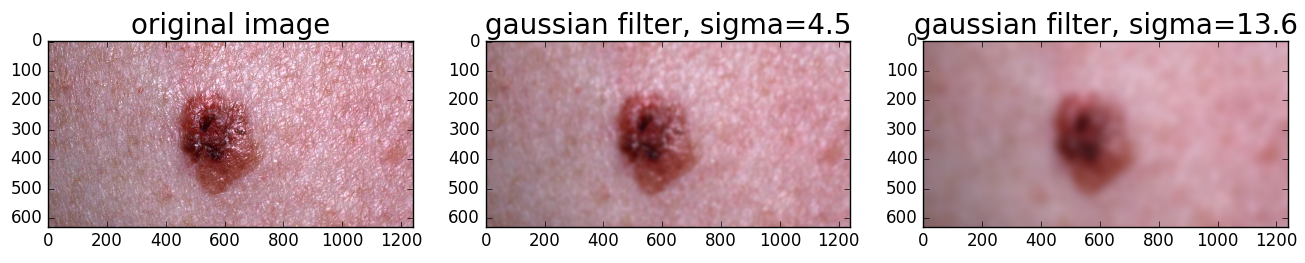
\includegraphics[width=\textwidth,keepaspectratio]{assets/image_processing/noise_reduction/gaussian/figure_01.png}
    \caption{Gaussian Filter Example A}
    \label{fig:med_A}
\end{figure}
\begin{figure}[H]
    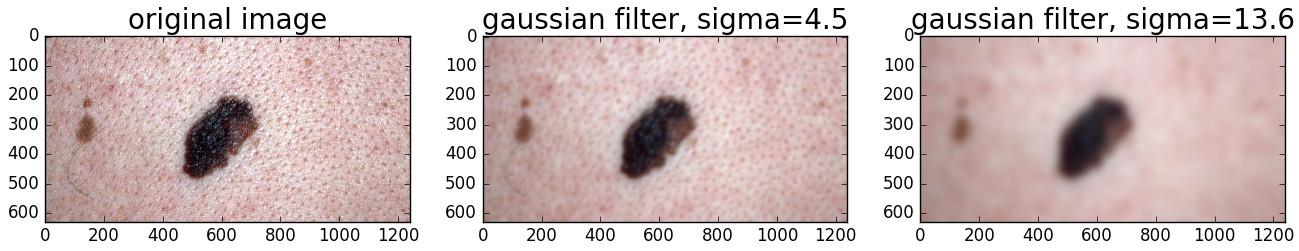
\includegraphics[width=\textwidth,keepaspectratio]{assets/image_processing/noise_reduction/gaussian/figure_02.png}
    \caption{Gaussian Filter Example B}
    \label{fig:med_B}
\end{figure}

In figure \ref{fig:med_B} there is a hair in the lower left side of the image. At higher sigma values the hair is still partially present, while the border of the lesion has already lost much detail. The tradeoff between noise reduction and loss of important detail is not optimal for the Gaussian filter.

\subsubsection{Median Filter}

The median filter will iterate through the pixels of an image, analysing each pixel and it's immediate neighbours. The value chosen for a pixels will be the median value of the area around the pixel. In a 2D context, if the neighbourhood around a pixel is [2,1,96] the pixel will receive the value 2. The median filter is easy to compute and has the quality that edges remain well preserved. This is therefore particularly useful as a preprocessing step before segmentation.

The following figures \ref{fig:med_A} to \ref{fig:med_C} are examples of median filtered images.

\begin{figure}[H]
    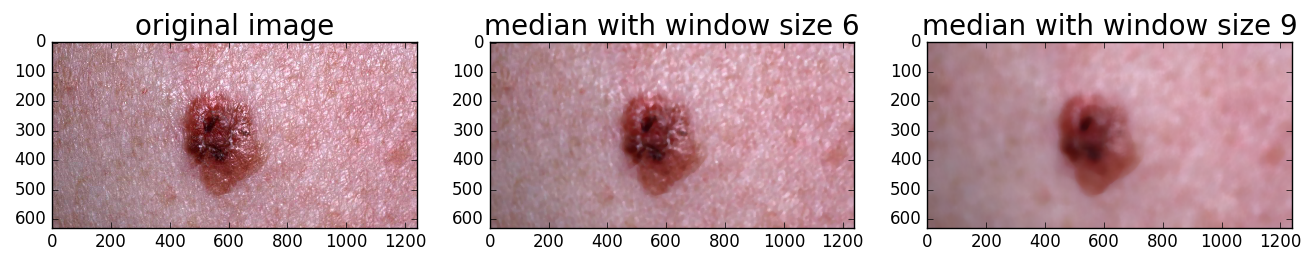
\includegraphics[width=\textwidth,keepaspectratio]{assets/image_processing/noise_reduction/figure_01.png}
    \caption{Median Filter Example A}
    \label{fig:med_A}
\end{figure}
\begin{figure}[H]
    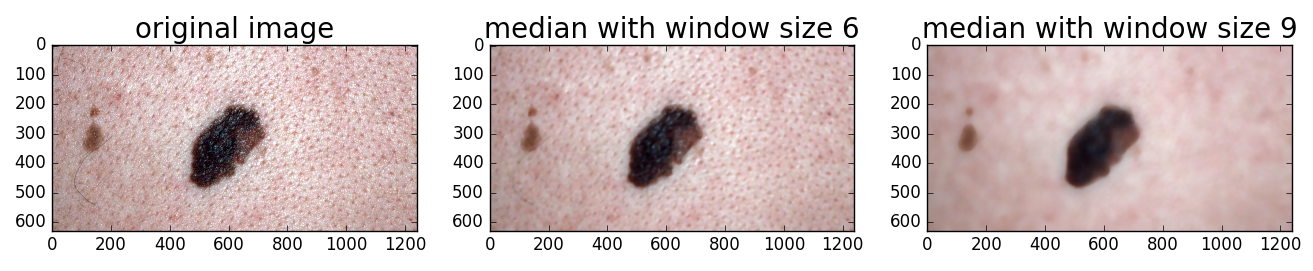
\includegraphics[width=\textwidth,keepaspectratio]{assets/image_processing/noise_reduction/figure_02.png}
    \caption{Median Filter Example B}
    \label{fig:med_B}
\end{figure}
\begin{figure}[H]
    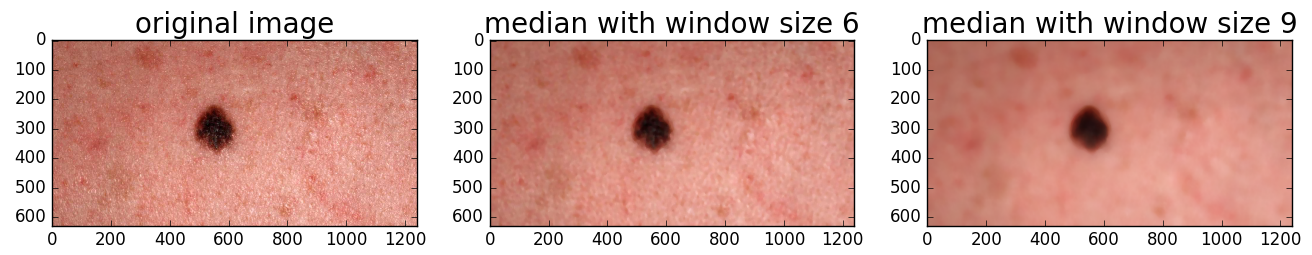
\includegraphics[width=\textwidth,keepaspectratio]{assets/image_processing/noise_reduction/figure_03.png}
    \caption{Median Filter Example C}
    \label{fig:med_B}
\end{figure}

The effect of the median window size is visible in the examples above. Larger window sizes are more effective at reducing noise and other disturbances. The edges of the lesion remain sharp, but the shape looses some detail, corners are rounded off. The size of the lesion in the image, and the image’s resolution are also important factors in the success of the median filter. If the lesion is too small compared to the image size, or the resolution of the image too low, then the shape will become more distorted. This will have a negative effect on the following segmentation steps.
\section{Segmentation}

\subsection{Iterative Thresholding}
\subsection{Region Selection}

\section{Image Feature Extraction}



\chapter{TDS Algorithm}
\section{Description of the Algorithm}

Early detection of melanoma greatly increases the chances of successful treatment. A biopsy can be performed in order to gain a definitive diagnosis. However, biopsies are invasive, painful and take time. There are also visual markers Dermatologists look for in order to make a risk assessment. The ABCD Rule, also known as Stokes or TDS Calculation, looks for 4 sets of features. Based on the features the Total Dermoscopy Score (TDS) is calculated.

The 4 sets of features are Asymmetry (A), Border Irregularity (B), Color (C) and Differential Structure or Diameter (D).

Asymmetry can have a value of 0, 1 or 2 depending on the symmetry of the lesion. Where 0 is symmetric and 2 is asymmetric. A value of 1 indicates at least one axis was found across which symmetry exists. The Border score is an integer value from 0 to 8 indicating the presence of border irregularities in 8 regions. Color is an integer value from 1 to 6 indicating the presence of one to six specific colors. Similarly, the value for D indicates the presence of one to five distinct structures or textures. Alternatively, in some literature\cite{Siddiq_2015} D is defined as Diameter, where a diameter greater than 6mm results in a value of 5, otherwise 1.

The final TDS Score is the weighted sum of the ABCD Values and is in the range 1.0 to 8.9.

\begin{equation}
TDS = A * 1.3 + B * 0.1 + C * 0.5 + D * 0.5
\end{equation}

A diagnosis can be made based on the TDS Score according to the following table:

\begin{table}[H]
\centering
\small
    \begin{tabular}{ | l | p{3.5cm} | l | p{3.5cm} |}
    \hline
    Evaluation & TDS Score \\ \hline
    Benign & \textless  4.75  \\ \hline
    Suspicious & 4.75 to 5.45  \\ \hline
    Malignant & \textgreater  5.45  \\ \hline

    \end{tabular}

    \caption{TDS Evaluation\cite{Weigert_2012}}
    \label{fig:tds_eval}

\end{table}


\section{Automatic Calculation of ABCD Values}

The ABCD Rule is used by Dermatologists to differentiate benign from malignant melanocytic tumors. Because it is a clearly defined rule based on easily recognizable visual features it is easy to apply. Clinicians with limited dermoscopy experience achieve better results using the ABCD rule than other methods \cite{Weigert_2012}. The following sections detail methods to automate the calculation of the ABCD scores.

\subsection{Asymmetry}

Asymmetry is a strong indicator of malignancy in a tumor. Of the 4 criteria in the ABCD rule, it is weighted highest.

\subsection{Border}

\subsection{Color}

\subsection{Differential}

\section{Two Examples}
\subsection{Postitiv Example}

\subsection{False Example}

ABCD Values were calculated but classification result was false.

\section{Results of Algorithm}

Performance Evaluation

Chapters 11.1, 11.2, maybe 11.3

\chapter{Machine Learning}
\section{Section Title}
\section{Results of Algorithm}

Performance Evaluation

Chapters from book 11.1, 11.2, 11.3, 11.5, 11.6

\chapter{Implementaion of the Algorithm}
\section{Section Title}

\chapter{Mobile App Requirements}
This chapter will describe the requirements of the application as a whole. The structure of this chapter follows the SRS Template as proposed by Wiegers in Chapter 11 and Appendix D of \cite{wiegers2013software}.

Table \ref{tab:ids} describes the idendifiers used to reference the requirement attributes descri

\begin{table}[H]
    \small
    \begin{tabular}[t]{ | l | p{3.5cm} | p{6.5cm} |} \hline

        \textbf{ID} & \textbf{Attribute} & \textbf{Description} \\ \hline
        FE-\# & Major Features & High level description of what the MDApp is expected to achieve. \\ \hline
        LI-\# & Limitations and Exclusions & Things that should not be considered part of the scope of the application \\ \hline
        UC-\# & Use Cases & Description of an activity that a user can perform. \\ \hline
        OE-\# & Operating Environment & Description of the environment the application will operate in. \\ \hline
        CO-\# & Design and Implementation Constraints & External technical factors that need to be taken account for. \\ \hline
        AS-\# & Assumptions and Dependencies & Other external factors or limitations that need to be considered. \\ \hline
        UI-\# & User Interfaces & Requirement that the user interface must fullfill. \\ \hline
        SI-\# & Software Interfaces & External software interfaces that the app must communicate with. \\ \hline
        CI-\# & Communication Interfaces & Description of communication interfaces. \\ \hline
        PRI-\# & Privacy & Privacy requirements. \\ \hline
        INS-\# & Installability & Installability requirements. \\ \hline
        INT-\# & Integrity & Data integrity requirements. \\ \hline
        USE-\# & Usability & Useability requirements. \\ \hline
        POR-\# & Portability & Portability requirements. \\ \hline
        TES-\# & Testability & Testability requirements. \\ \hline

    \end{tabular}
    \caption{List of attribute identifiers}
    \label{tab:ids}
\end{table}

\section{Vision and Scope}

    This section describes the high levels goal of the Melanoma Detection App as well as to define boundaries that limit what can be expected of the App.

    \subsection{Business Case}

        A smart phone based assistant would provide a valuable service by making it easy, painless, inexpensive, and fast to get a preliminary risk assessment of a skin lesion. It is too easy to postpone making an appointment with a dermatologist to have a suspect lesion examined. Visiting a dermatologist is not on most people’s list of fun things to do, it requires time and effort. By the time a lesion is visually compelling enough, it might be too late.

A smart phone based application that could make a preliminary diagnosis in near realtime would be a great time save and offer compelling enough information to actually make the appointment with a dermatologist.

    \subsection{Scope and Limitations}

    This chapter describes which features are part of the scope of the Melanoma Detection Application, what can be expected of it, and what are it's limitations.

    \subsubsection{Major Features}
        \noindent
        \begin{itemize}[leftmargin=*]
            \item[]  \textbf{FE-1} : The smart phone app allows the user to capture and analyse an image of a skin lesion and provide a risk assessment to the user of the lesion being a malignant melanoma.

            \item[] \textbf{FE-2} : The app allows the user to create, view, edit or delete metadata that is associated with an image and corresponding risk assessment.

            \item[] \textbf{FE-3} : The app allows the user to save or archive the image and corresponding assessment for future comparison and review.

            \item[] \textbf{FE-4} : The user can browse archived images, assessments, and associated metadata.

            \item[] \textbf{FE-5} : The user can send a set of images with associated assessment and metadata via email.

            \item[] \textbf{FE-6} : The app will run on all popular smart phone devices and systems.

            \item[] \textbf{FE-7} : The analysis algorithms employed by the app should be easily updatable and extendable.
        \end{itemize}

        \begin{figure}[H]
            \centering
            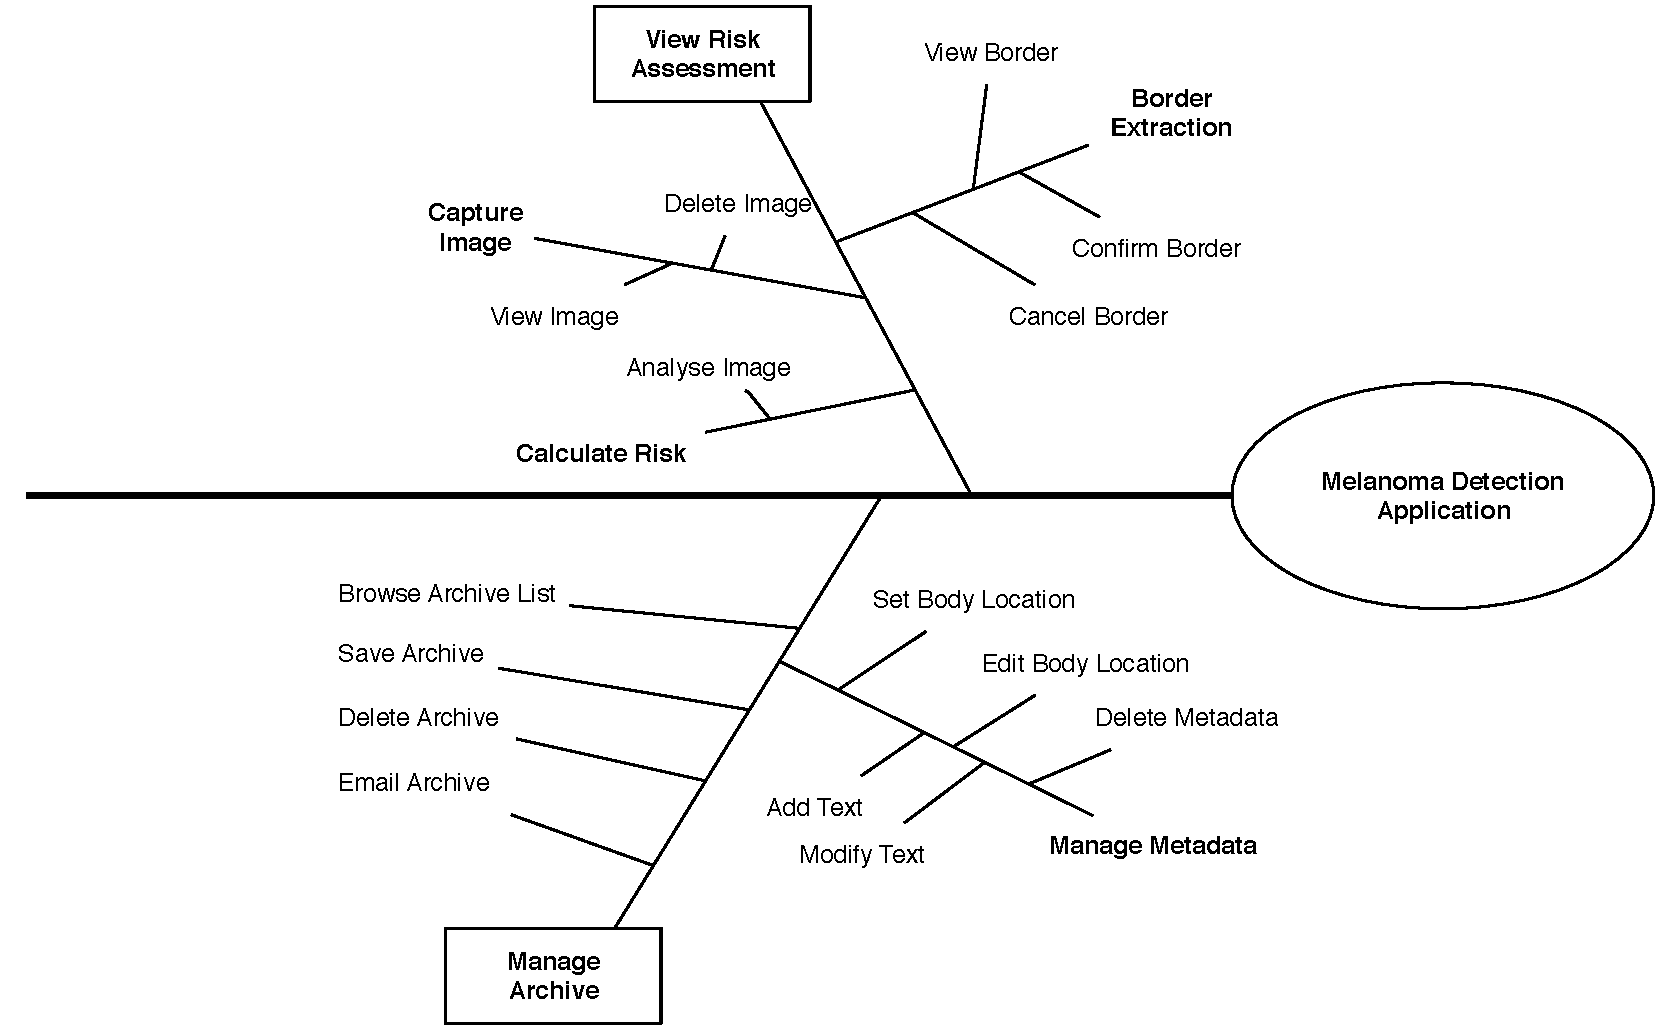
\includegraphics[width=\textwidth]{assets/requirements/PartialFeatureTree.pdf}
            \caption{Partial Feature Tree for the Melanoma Detection App}
            \label{fig:partial_feature_tree}
        \end{figure}

    \subsubsection{Limitations and Exclusions}

        \noindent
        \begin{itemize}[leftmargin=*]
            \item[]  \textbf{LI-1} : The Melanoma Detection App will use visual indicators to calculate the risk of a lesion being a dangerour melanoma. Other types of skin cancer such as basal call carcinoma or squanous cell carcinoma have different characteristics making them less easy to visually detect. The Melanoma Detection App will not take any other types of skin cancer or skin conditions into acount when calculating the risk assessment for melanoma.
            \item[]  \textbf{LI-2} : Typical Smartphone camera's might not have the ability to capture images at close enough range needed to capture a skin lesion's details at high enough resolution. It might be necessary for the Smartphone User to additionaly purchase a readily available clip-on macro lens for smart phones.

        \end{itemize}

    \subsubsection{Stakeholder Profile}

        % TODO

    \subsection{Use Cases}

        10 Important Use Cases have been identified. The schema as defined in Chapter 8 and Appendix D of \cite{wiegers2013software} was used to capture the attributes of each Use Case. The Use Case UML diagram in figure \ref{fig:uml} illustrates the most important use cases. Tables \ref{fig:uc-1} to \ref{fig:uc-10} describe the use cases in detail.

        \begin{figure}[H]
            \centering
            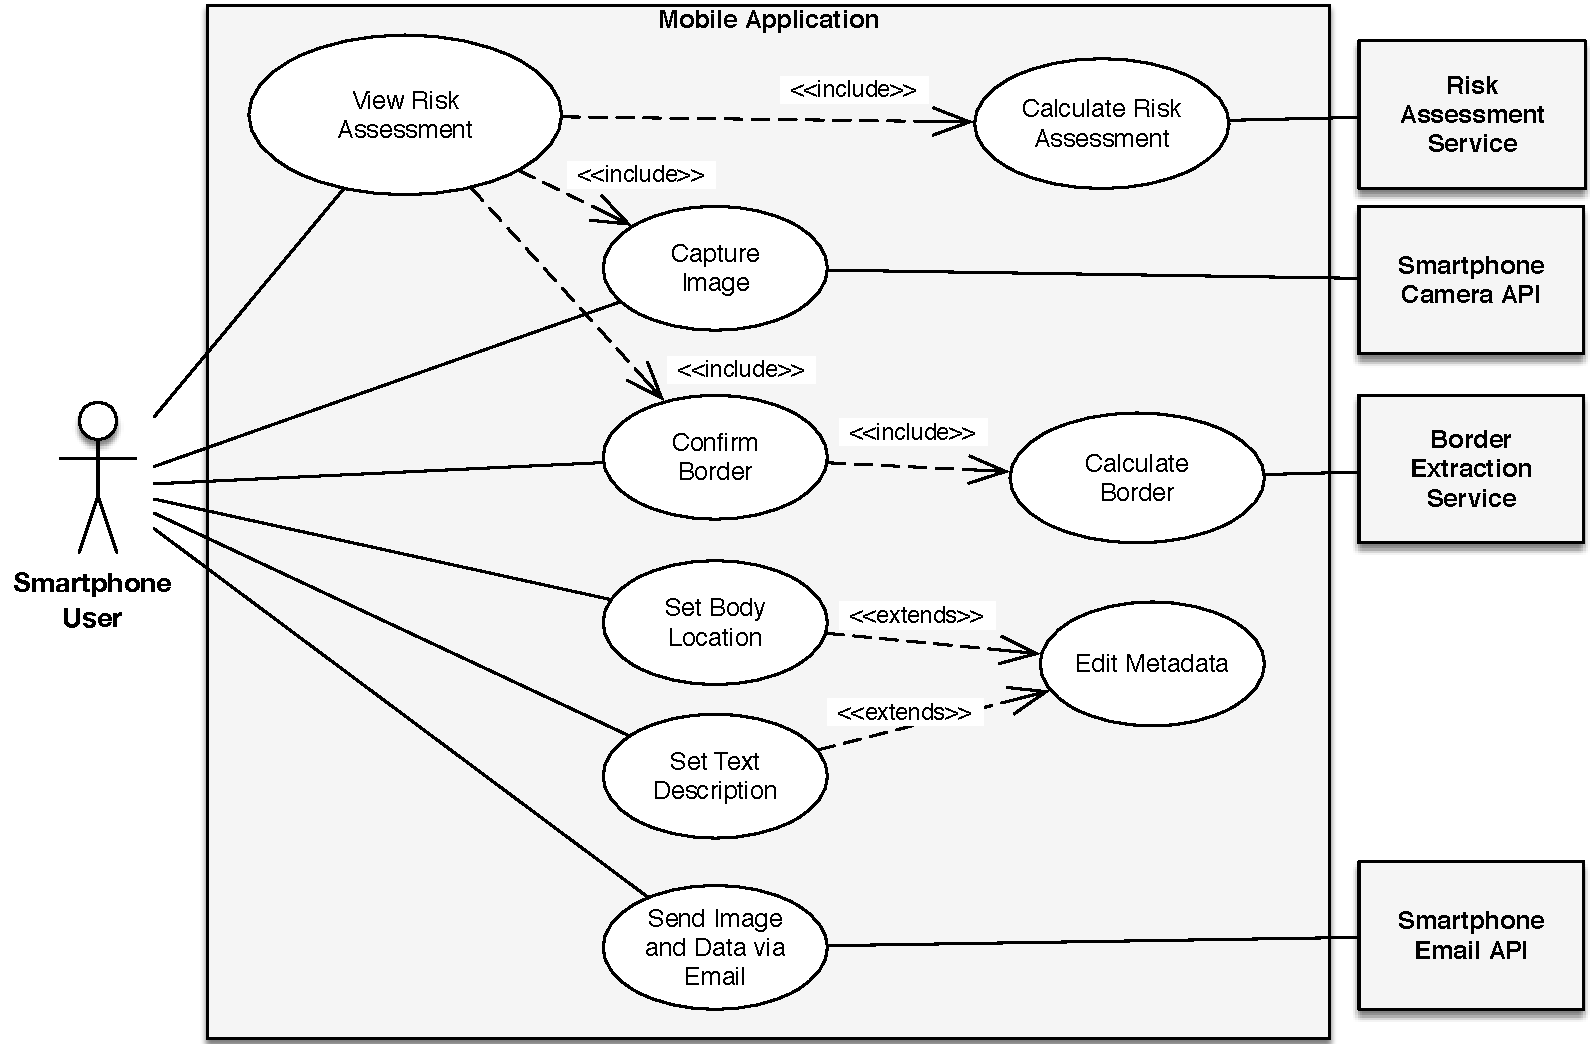
\includegraphics[width=\textwidth]{assets/requirements//uc/UML.pdf}
            \caption{Use Case UML diagram}
            \label{fig:uml}
        \end{figure}

                \begin{table}[H]
            \centering
            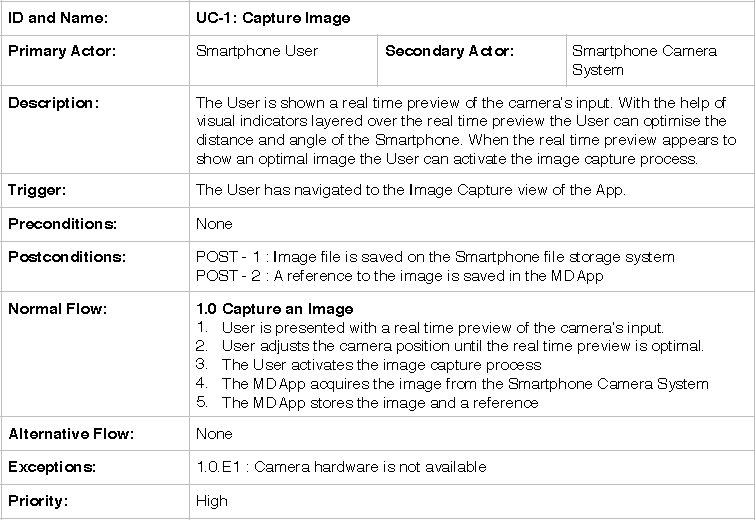
\includegraphics[width=\textwidth]{assets/requirements/uc/usecase_01.pdf}
            \caption{UC-1}
            \label{fig:uc-1}
        \end{table}
        \begin{table}[H]
            \centering
            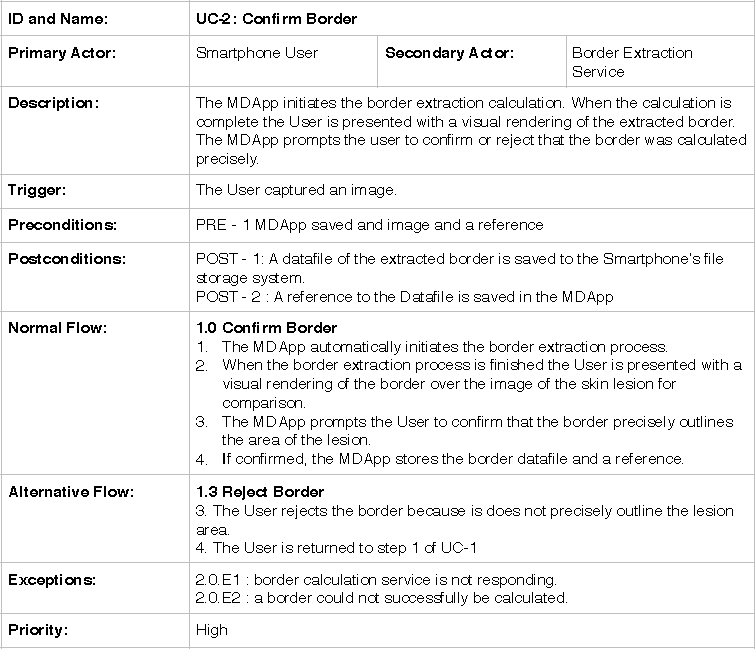
\includegraphics[width=\textwidth]{assets/requirements/uc/usecase_02.pdf}
            \caption{UC-2}
            \label{fig:uc-2}
        \end{table}
        \begin{table}[H]
            \centering
            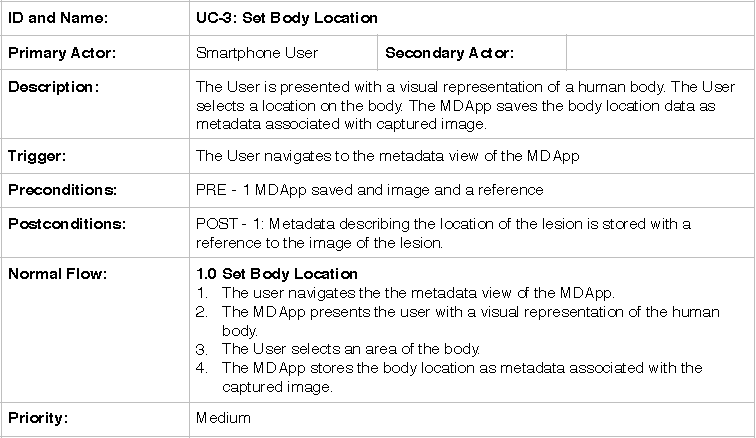
\includegraphics[width=\textwidth]{assets/requirements/uc/usecase_03.pdf}
            \caption{UC-3}
            \label{fig:uc-3}
        \end{table}
        \begin{table}[H]
            \centering
            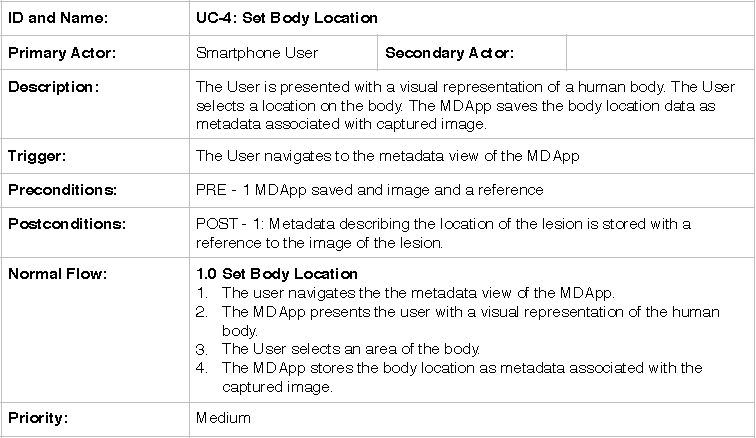
\includegraphics[width=\textwidth]{assets/requirements/uc/usecase_04.pdf}
            \caption{UC-4}
            \label{fig:uc-4}
        \end{table}
        \begin{table}[H]
            \centering
            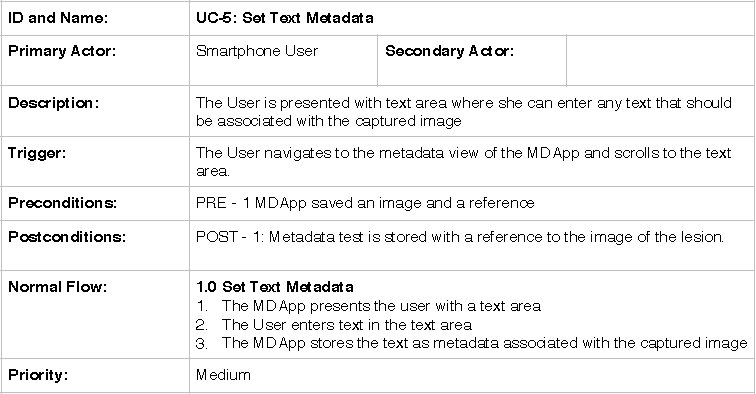
\includegraphics[width=\textwidth]{assets/requirements/uc/usecase_05.pdf}
            \caption{UC-5}
            \label{fig:uc-5}
        \end{table}
        \begin{table}[H]
            \centering
            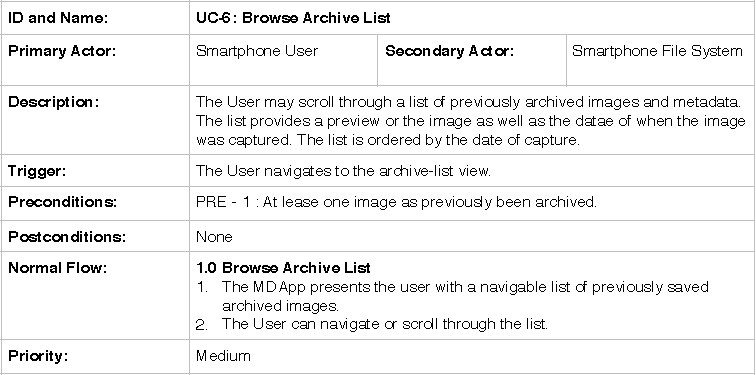
\includegraphics[width=\textwidth]{assets/requirements/uc/usecase_06.pdf}
            \caption{UC-6}
            \label{fig:uc-6}
        \end{table}
        \begin{table}[H]
            \centering
            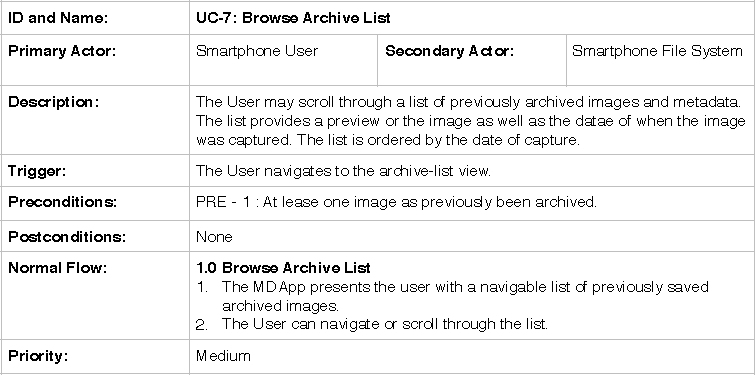
\includegraphics[width=\textwidth]{assets/requirements/uc/usecase_07.pdf}
            \caption{UC-7}
            \label{fig:uc-7}
        \end{table}
        \begin{table}[H]
            \centering
            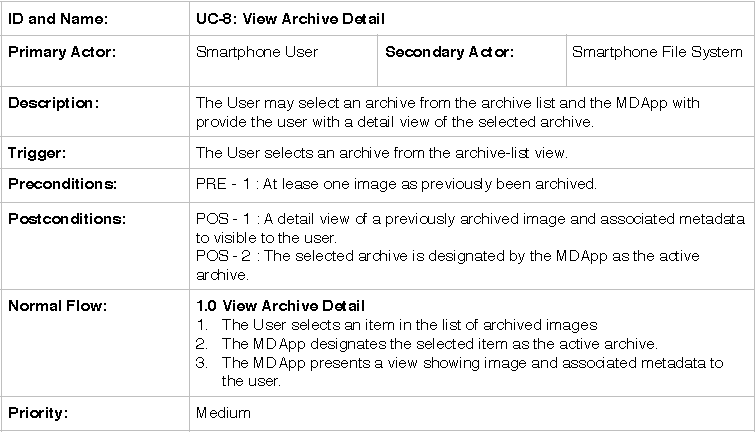
\includegraphics[width=\textwidth]{assets/requirements/uc/usecase_08.pdf}
            \caption{UC-8}
            \label{fig:uc-8}
        \end{table}
        \begin{table}[H]
            \centering
            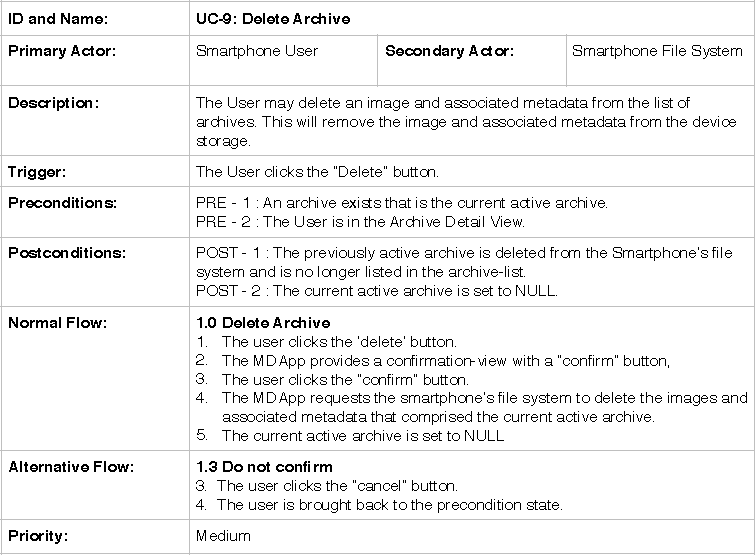
\includegraphics[width=\textwidth]{assets/requirements/uc/usecase_09.pdf}
            \caption{UC-9}
            \label{fig:uc-9}
        \end{table}
        \begin{table}[H]
            \centering
            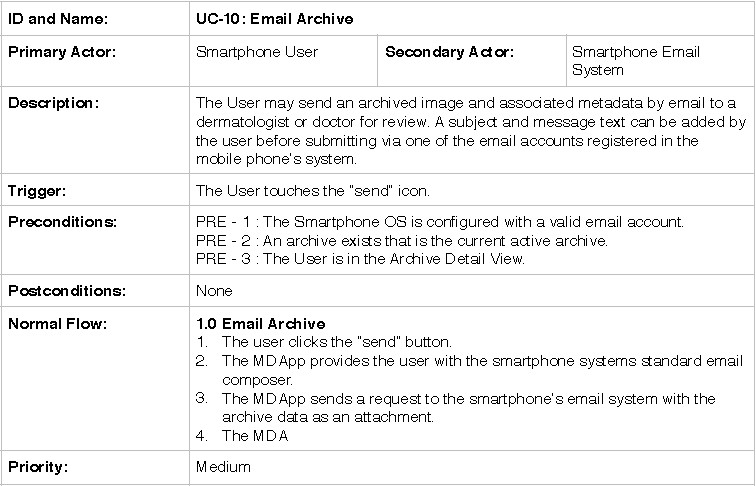
\includegraphics[width=\textwidth]{assets/requirements/uc/usecase_10.pdf}
            \caption{UC-10}
            \label{fig:uc-10}
        \end{table}



\section{Software Requirements Specification}

    \subsection{Introduction}
        \subsubsection{Purpose}

            The Software Requirements Specification will describe the functional and nonfunctional requirements of the Melanoma Detection App. It is meant to be a guideline for developers who will be implementing the mobile application.

    \subsection{Overall Description}
        
        \subsubsection{Product Perspective}

            The Melanoma Detect App will provide the user with a risk assessment of a skin lesion. The App will guide the user through the process of capturing an image and confirming the correct recognition of the boundary of the lesion. Once confirmed the App will analyse the visual features of the lesion based on dermatological rules and provide the user with an initial risk assessment.

    The App should help motivate the user to make an appointment with a dermatologist when a significant risk has been detected. It is not meant to replace the need to visit a dermatologist though.


            \begin{figure}[H]
                \centering
                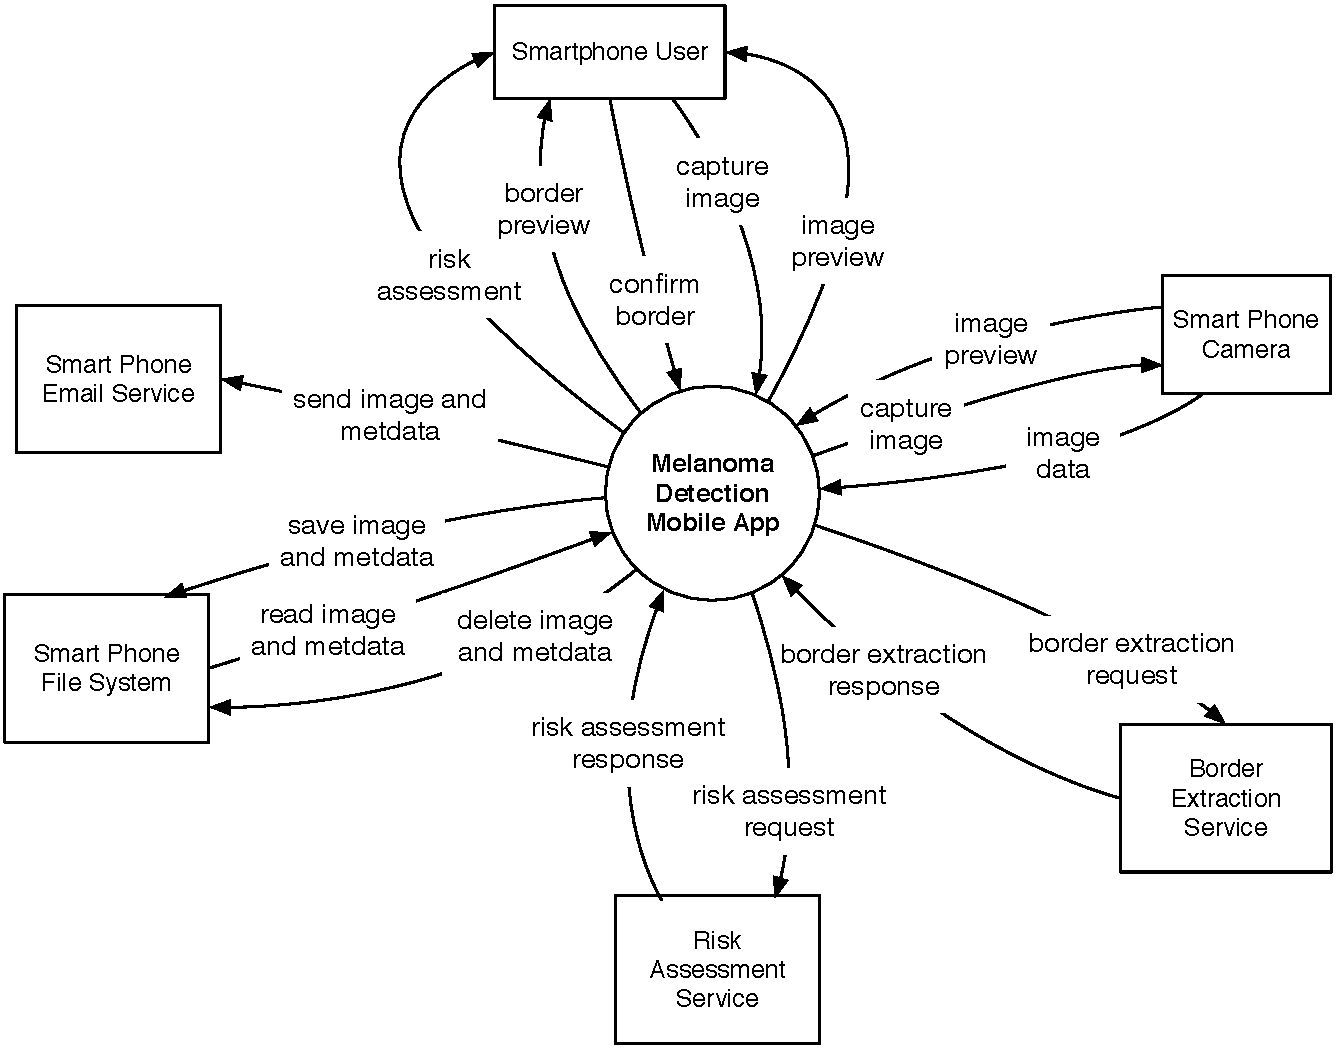
\includegraphics[width=\textwidth]{assets/requirements/ContextDiagram.pdf}
                \caption{Context Diagram of the Melanoma Detection App}
                \label{fig:partial_feature_tree}
            \end{figure}


        \subsubsection{User Classes and Characteristics}

            The Melanoma Detection App only has one class of user, the Smartphone User. The Smartphone User has one or several skin lesions that she or he is worried about.
The Smartphone User is not expected to have any technical or dermatological expertise.

        \subsubsection{Operating Environment}

                    \noindent
                    \begin{itemize}[leftmargin=*]
                        \item[]  \textbf{OE-1} : The Mobile App shall operate on the following platforms: Android OS (minumum v.5.2.2) and iOS (minumum v.9.3)

                    \end{itemize}


        \subsubsection{Design and Implementation Constraints}

                    \noindent
                    \begin{itemize}[leftmargin=*]
                        \item[]  \textbf{CO-1} : The Border Extraction and Risk Assessment Services shall be implemented on a server in oder to leverage the effort already made with python and python based libraries for image processing and scientific calculations. Wifi access is therefore a requirement for the app to run.
                        \item[]  \textbf{CO-2} : The method for archiving images and risk assessment data will use whatever standard is the most accepted for the relevant platform. i.e. iCloud on iOS.


                    \end{itemize}

        \subsubsection{Assumptions and Dependencies}

                    \noindent
                    \begin{itemize}[leftmargin=*]
                        \item[]  \textbf{AS-1} : It is assumed that the user of the software is also the user of the mobile phone. The software might need to request permission from the user to access the camera or network.

                    \end{itemize}

                    \noindent
                    \begin{itemize}[leftmargin=*]
                        \item[]  \textbf{AS-2} : It is assumed that the user of the software is also the only user of the mobile phone. Therefore no additional measures need be taken to secure the app from other potiential users of the phone. The app will be as secure as the phone itself.

                    \end{itemize}

    \subsection{System Features}
        {\renewcommand{\arraystretch}{1.8}%

        \subsubsection{Capture an Image of a Skin Lesion}
            \paragraph{Description}

            The MDApp allows the Smartphone User to capture an image of a skin lesion.

            \paragraph{Functional Requirements}



                \begin{longtable}[H]{ >{\bfseries}l >{\bfseries}l >{\bfseries}l p{8.5cm} l }

                    \hline
                    & \multicolumn{2}{>{\bfseries}l}
                    {Image.Capture:} & \textbf{Capture image using camera}  \\

                    & & .Preview: &  The App must provide the User with a realtime preview of the camera input. It will include some visual indicators that help the user capture an optimal image. \\

                    & & .Trigger: & The User will trigger the capture when he or she decides the realtime preview is optimal. \\

                    & & .Response: & The App must be able to capture a still image from the camera when the User pushed the capture button. The image will be saved in a standard image format on the phone’s file system. \\

                    & & .Display: & The App will present the image to the user on the device’s screen. \\

                    \hline
                \end{longtable}


        \subsubsection{Extract the Border of a Skin Lesion}

            \paragraph{Description}

            In oder to be able to properly analyse the skin lesion image, the MDApp must be able to distinguish pixels that belong to the lesion from pixels that belong to the healthy skin area surrounding the lesion.

            \paragraph{Functional Requirements}

                \begin{longtable}[H]{ >{\bfseries}l >{\bfseries}l >{\bfseries}l >{\bfseries}l p{8.5cm} l }

                    \hline
                    & \multicolumn{3}{>{\bfseries}l}
                    {Border.Extract:} & \textbf{Calculate border of skin lesion}  \\

                    & & \multicolumn{2}{>{\bfseries}l}{.Calculate:} &
                    The App sends a captured image as a request to the Border Extraction Service. When the service has completed the calculation the results of the border calculation are provided by the service to the App.
                    \\

                    & & & .NA & %TODO
                    \\

                    & & & .Err & %TODO
                    \\

                    & & \multicolumn{2}{>{\bfseries}l}{.Display:} &
                    The App will present the results or the border calculation to the User on the device’s screen.
                    \\

                    & & \multicolumn{2}{>{\bfseries}l}{.Promt:} & The App will prompt the User to confirm that the border was precisely calculated. \\

                    & & \multicolumn{2}{>{\bfseries}l}{.Response:} & The User can confirm or cancel the border. \\

                    \hline
                \end{longtable}


        \subsubsection{Calculate the Risk Assessment Skin Lesion}

            \paragraph{Description}

            The MDApp sends the skin lesion image and border data as a request to the Risk Assessment Service.

            \paragraph{Functional Requirements}
                \begin{longtable}[H]{ >{\bfseries}l >{\bfseries}l >{\bfseries}l p{8.5cm} l }

                    \hline
                    & \multicolumn{2}{>{\bfseries}l}
                    {Risk.Assessment:} & \textbf{Calculate risk assessment of lesion image}  \\

                    & & .Calculate: &
                    The App sends a captured image and border data as a request to the Risk Assessment Service. When the service has completed the calculation the results of the risk assessment are provided by the service to the App.
                    \\

                    & & .Display: &
                    The App will present the results or the risk assessment calculation to the User on the device’s screen.
                    \\
                    \hline
                \end{longtable}


        \subsubsection{Create, Modify, and Delete Metadata}

            \paragraph{Description}

            The Smartphone User can add metadata to a captured image. This can include the location on the body that the image was captured from, date of capture, and a text description. This metadata can be associated with an image so that it can be used at a later data for comparison and review.

            \paragraph{Functional Requirements}
                \begin{longtable}[H]{ >{\bfseries}l >{\bfseries}l >{\bfseries}l p{8.5cm} l }

                    \hline

                    & \multicolumn{2}{>{\bfseries}l}
                    {Metadata.Location:} & \textbf{Specify the lesion’s location on body}  \\

                    & & .Display: &
                    The MDApp will present an image of the human body to the Smartphone User.
                    \\

                    & & .Promt: &
                    The MDApp will prompt the Smartphone User to select or zoom in on a location on the image of the human body.
                    \\

                    & & .Response: &
                    The selected location will be stored as metadata associated with the image of the lesion.
                    \\
                    \hline

                    & \multicolumn{2}{>{\bfseries}l}
                    {Metadata.Text:} & \textbf{Add metadata describing lesion}  \\

                    & & .Display: &
                    The MDApp will present a text field in which the Smartphone User may enter, edit, or delete text.
                    \\


                    & & .Response: &
                    The entered text will be stored as metadata associated with the image of the lesion.
                    \\

                    \hline
                \end{longtable}


        \subsubsection{Save, View, Edit, Delete and Email Archive}


            \paragraph{Description}

            The Smartphone User can browse a list of previously analysed and saved images (archives). From the list, an image may be selected by the Smartphone User to view in more detail. When selected the MDApp will present the saved image, border, risk assessment, and associated metadata to the Smartphone User for review. An archive from the list may also be deleted or sent as an email.

            \paragraph{Functional Requirements}
                \begin{longtable}[H]{ >{\bfseries}l >{\bfseries}l >{\bfseries}l p{8.5cm} l }

                    \hline

                    & \multicolumn{2}{>{\bfseries}l}
                    {Archive.Save:} & \textbf{Save image and metadata as archive}  \\

                    & & .Display: &
                    ---
                    \\
                    \hline
                    & \multicolumn{2}{>{\bfseries}l}
                    {Archive.Browse:} & \textbf{Browse list of archived images}  \\

                    & & .Display: &
                    The MDApp will present the Smartphone User with a list of saved archive images.
                    \\
                    \hline
                    & \multicolumn{2}{>{\bfseries}l}
                    {Archive.Select:} & \textbf{Select archived image to view or edit}  \\

                    & & .Display: &
                    The MDApp will present the Smartphone User with a detail view of the selected archived image and associated metadata.
                    \\
                    & & .Edit: &
                    The MDApp will present a text field in which the Smartphone User may enter, edit, or delete text.
                    \\
                    & & .Delete: &
                    The MDApp will present a text field in which the Smartphone User may enter, edit, or delete text.
                    \\
                    & & .Email: &
                    The MDApp will present a text field in which the Smartphone User may enter, edit, or delete text.
                    \\


                    \hline
                \end{longtable}
}



    \subsection{Data Requirements}
        
        \subsubsection{Logical Data Model}

            \begin{figure}[H]
                \centering
                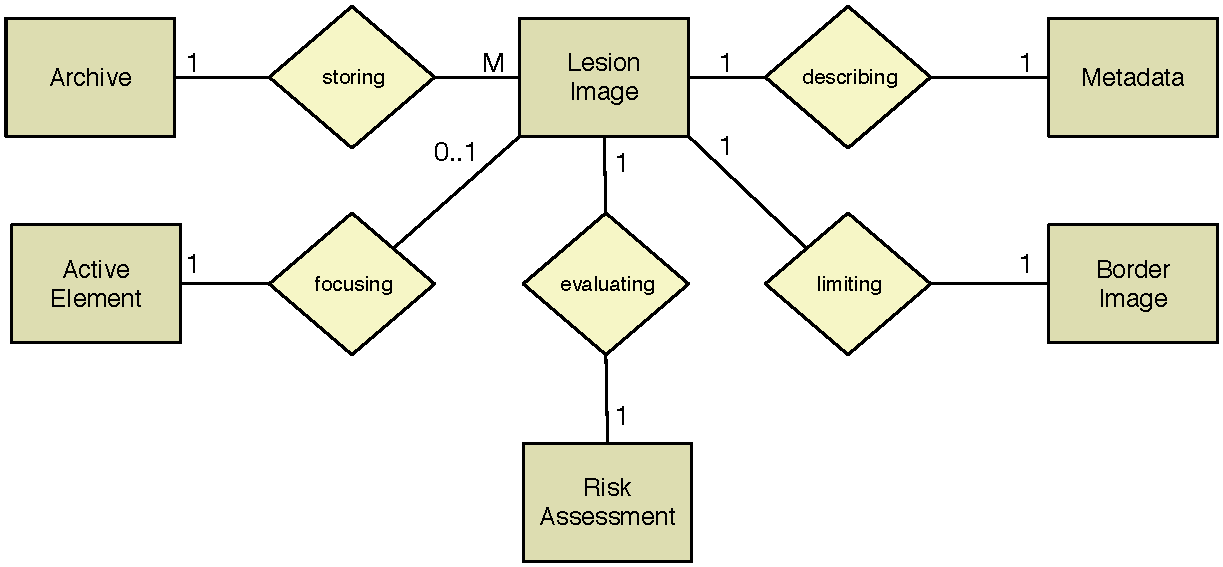
\includegraphics[width=\textwidth]{assets/requirements/EntRel.pdf}
                \caption{Patial data model of the Melanoma Detection App}
                \label{fig:partial_data_model}
            \end{figure}


        \subsubsection{Data Dictionary}

                \begin{longtable}[H]{ | l | p{3.0cm} | p{2.5cm} | p{1.0cm} | p{2.5cm} | }

                    \hline
                    \textbf{Data element} & \textbf{Description} & \textbf{Componsition or data type} & \textbf{Length} & \textbf{Values} \\ \hline

                    \hypertarget{lesion_image}{Lesion Image} & reference to the captured image &

                        \specialcell[t]{Image ID
                           \\ + File Path
                           \\ + Creation Date
                        }

                     & & \\ \hline

                    Image ID & unique identifier for an image &
                    integer & 11 & system-generated sequential integer beginning with 1 \\ \hline

                    File Path & location of a file on the file system &
                    string & 256 &  \\ \hline

                    Creation Date & date and time that a file was created &
                    DDMMYYYYHHSS &  &  \\ \hline

                    Metadata & information describing the lesion and it's location &

                        \specialcell[t]{\hyperlink{lesion_image}{Lesion Image}
                           \\ + Lesion Description
                           \\ + Lesion Location
                        }

                     & & \\ \hline

                    Lesion Description & User defined text that describes the lesion &
                    alphanumeric &  &  \\ \hline

                    Lesion Location & information describing the lesion location on the body &

                        \specialcell[t]{\hyperlink{lesion_image}{Lesion Image}
                           \\ + Body Location ID
                           \\ + X Coordinate
                           \\ + Y Coordinate
                        }

                     & & \\ \hline


                    Body Location ID & id of a region on the body &
                    integer & 2 & TBD \\ \hline

                    X Coordinate & x coordinate of the lesion in the region specified by the body location id &
                    integer & 128 &  \\ \hline

                    Y Coordinate & y coordinate of the lesion in the region specified by the body location id &
                    integer & 128 &  \\ \hline

                    Border Image & data that defines the outline of the lesion area &

                        \specialcell[t]{\hyperlink{lesion_image}{Lesion Image}
                           \\ + File Path
                           \\ + Creation Date
                        }

                     & & \\ \hline

                    Risk Assessment &  &

                        \specialcell[t]{\hyperlink{lesion_image}{Lesion Image}
                            \\ + Assessment Date
                            \\ + Version Number
                            \\ + SFA Major
                            \\ + SFA Minor
                            \\ + Border Irregularity
                            \\ + Color Score
                            \\ + \hyperlink{tds_score}{TDS Score}
                        }

                    & & \\ \hline

                    Assessment Date & date and time that the risk assessment was calculated &
                    DDMMYYYYHHSS &  &  \\ \hline

                    Version Number & version number of the risk assessment service software &
                    integer & 4 &  \\ \hline

                    SFA Major & measure of symmetry of the lesions major axis &
                    integer & 3 & 0 - 360 \\ \hline

                    SFA Minor & measure of symmetry of the lesions minor axis &
                    integer & 3 & 0 - 360 \\ \hline

                    Border Irregularity & measure of irregulatiry of the lesion's border &
                    integer & 1 & 0 - 8 \\ \hline

                    Color Score & number of specific colors found in the lesion's image &
                    integer & 1 & 0 - 8 \\ \hline

                    \hypertarget{tds_score}{TDS Score} & weighted linear combination of the image features summarizing the risk assessment  &
                    float &  & 1 - 8.9 \\ \hline

                    Archive &  &

                        \specialcell[t]{Archive ID
                            \\ + \hyperlink{lesion_image}{Lesion Image}
                            \\ + Metadata
                            \\ + Border
                            \\ + Risk Assessment
                            \\ + Archive Date
                        }

                     & & \\ \hline


                    Color Score & number of specific colors found in the lesion's image &
                    integer & 1 & 0 - 8 \\ \hline

                \end{longtable}


        \subsubsection{Data analysis}
            \paragraph{CRUD Matrix}

                \begin{figure}[H]
                    \centering
                    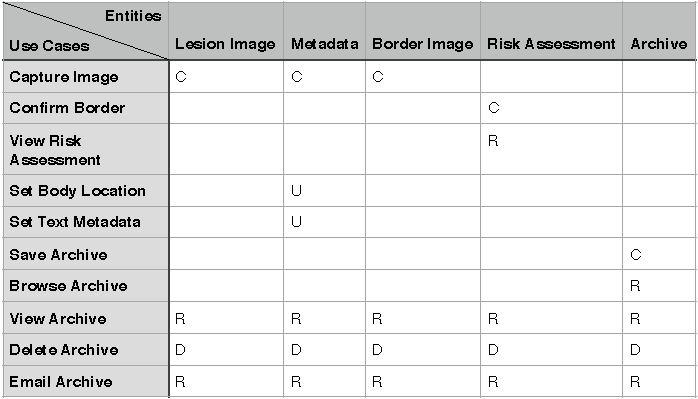
\includegraphics[width=\textwidth]{assets/requirements/CRUD.pdf}
                    \caption{CRUD matrix for Melanoma Detection App}
                    \label{fig:crud}
                \end{figure}

        \subsubsection{Reports}
            \paragraph{Email Report}
                When the Smartphone User chooses to send an archive as an email, the data must be flattened into a format that is email compatible. The body of the email will be an html formated document that displays the lesion image, the calculated border, the risk assessment data and the associated metadata.




    \subsection{External Interface Requirements}
        \subsubsection{User Interfaces}

        \begin{itemize}[leftmargin=1.4cm]
            \item[UI-1 :] The UI shall guide the Smartphone User sequentially through the process of capturing and analysing an image. The Smartphone User should not be able to jump through states in wrong sequence.
            \item[UI-2 :] The UI shall allow the Smartphone User to capture an image easily, using only one hand.
            \item[UI-3 :] When waiting for a process to finish or a response from an online server the UI should visually indicate that it is waiting for a long process. ( i.e. throbber, spinning wheel, progress indicator )
            \item[UI-4 :] The UI shall allow the Smartphone User to select her or his preferred language ( i.e. localisation )
            \item[UI-5 :] The UI shall conform to native UI standards as much as possible.
            \item[UI-6 :] Unless in conflict with UI-5 the UI shall have the same components across multiple platforms.

        \end{itemize}

\subsubsection{Software Interfaces}

    \paragraph{Smartphone Camera }

        The MDApp will interface with the Smartphone's camera hardware via the systems camera API.

        \begin{itemize}[leftmargin=1.4cm]
            \item[SI-1.1 :] The MDApp shall activate the camera when needed and be able to receive a live preview stream from the camera.
            \item[SI-1.2 :] If the native API allows, the MDApp should set to camera’s focus mode to Macro.
            \item[SI-1.3 :] If the native API allows, the MDApp should register a call back to be informed when the camera’s autoFocus has focused.
            \item[SI-1.4 :] The MDApp shall signal the camera to capture the highest resolution image possible when the Smartphone User triggers an image capture event.

        \end{itemize}

    \paragraph{Smartphone File System}

        Captured images and Border Analysis images must be stored on the Smartphone File System in such a manner so that they are accessible by the Smartphone User in the native methods. The native file access, file handling, and backup methods for the respective Smartphone platform shall apply to files created and captured by the MDApp

        \begin{itemize}[leftmargin=1.4cm]
            \item[SI-2 :] The MDApp will save files to the Smartphone's native file system.

        \end{itemize}

    \paragraph{Smartphone Email Service}

            \begin{itemize}[leftmargin=1.4cm]
            \item[SI-3 :]

        \end{itemize}

\subsubsection{Communication Interfaces}

    \paragraph{Border Extraction Service }

        The Border Extraction Service is an online web based service that the MDApp can communicate with for the purpose of extracting the precise border information from a captured image of a skin lesion.

        \begin{itemize}[leftmargin=1.4cm]
            \item[CI-1.1 :] The MDApp will upload a captured skin lesion image to a web-based Border Extraction Service. The method for uploaded as part of a multipart/form-data html POST method.
            \item[CI-1.2 :] The MDApp will receive a confirmation from the service as JSON, including an id that will be used to poll the service for progress.
            \item[CI-1.3 :] The MDApp will poll the online service regularly, the service will indicated that the Border Extraction processes is in progress or has finished, in which case it will also include the url where the border image can be downloaded.
            \item[CI-1.4 : ] The MDApp will download the border data image from the Border Extraction Service

        \end{itemize}

    \paragraph{Risk Assessment Service }

        The Risk Assessment Service is an online web based service that the MDApp can communicate with for the purpose of evaluating the risk of a skin lesion being a melanoma.

        \begin{itemize}[leftmargin=1.4cm]
            \item[CI-2 :] The MDApp will upload a captured skin lesion image to a web-based Border Extraction Service. The method for uploaded as part of a multipart/form-data html POST method.

        \end{itemize}

    \subsection{Quality Attributes}

        This section lists and describes the non-functional requirements.

        \subsubsection{External Quality Attributes}

            \paragraph{Privacy}

                \begin{itemize}[leftmargin=1.4cm]
                    \item[PRI-1 :] No information about the user shall be transmitted to any external services with the exception of when the user sends the image and metadata via email.
                \end{itemize}

            \paragraph{Installability}

                \begin{itemize}[leftmargin=1.4cm]
                    \item[INS-1 :] Installing the MDApp shall not require any special instructions other than those a normal Smartphone User would expect.
                \end{itemize}

            \paragraph{Integrity}

                \begin{itemize}[leftmargin=1.4cm]
                    \item[INT-1 :] Any data created by the Smartphone User through use of the MDApp shall be backup-able through whatever native backup solutions the native platoform offers.
                    \item[INT-2 :] Data and state shall be persisted, so that when reopened, the MDApp will have the same state as when it was last closed.
                    \item[INT-3 :] Data and state shall be persisted, so that no data is lost when the MDApp is updated.
                \end{itemize}

            \paragraph{Usability}

                \begin{itemize}[leftmargin=1.4cm]
                    \item[USE-1 :] Every function on the MDApp can be completed with one hand.
                \end{itemize}

        \subsubsection{Internal Quality Attributes}

            \paragraph{Portability}

                \begin{itemize}[leftmargin=1.4cm]
                    \item[POR-1 :] The MDApp's system features shall be implemented accross all the device platforms it runs on.
                \end{itemize}

            \paragraph{Testability}

                \begin{itemize}[leftmargin=1.4cm]
                    \item[TES-1 :] Individual components of the system must be testable in isolation from one another.
                    \item[TES-2 :] Tests shall be implemented in a manner allowing compontents to be tested automatically and test converage to be tracked.
                \end{itemize}


        \subsubsection{Quality Attribute Prioritisation}

            Depending on the domain of an application quality attributes might vary in importance. Prioritising the attributes will help in making descisions regarding the architecture and design of an application. Choosing a framework that targets achieving high performance may have a negative impact on portability, if portability has a high priority, then alternative frameworks should be considered. In figure \ref{fig:qa_prio} the quality attributes are compared pair-wise and tallied.

            \begin{figure}[H]
                \centering
                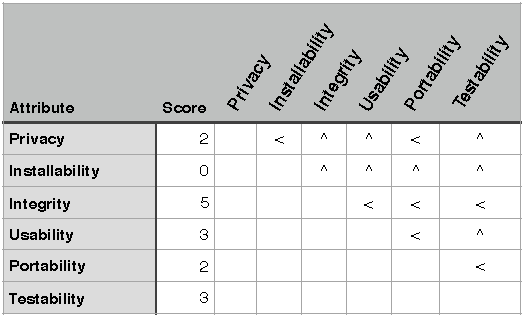
\includegraphics[width=8cm]{assets/requirements/QualityPrio.pdf}
                \caption{Prioritisation of Quality Attributes}
                \label{fig:qa_prio}
            \end{figure}





\chapter{Architecture Design}

\section{Software Architecture}
\subsection{MVC}
Since the 1970s the Model View Controller ( MVC ) pattern is the standard architectural design pattern for applications that present the user with a graphical user interface. It was developed out of a need for modularity, to encapsulate responsibility of specific concepts to separate program modules, or Separation of Concerns. MVC identifies three main components that program code should be grouped into, namely\cite{walther_2016}:

\begin{itemize}[label={}]

\item \textbf{Model}: The representation of some object of knowledge, encapsulates code managing the associated data and behaviour ( business-logic ).
\item \textbf{View}: The visual representation of the model. The view can feature or hide aspects of the model and thus act as a presentation filter. The view observe the model for changes and update the presentation accordingly.
\item \textbf{Controller}: The controller allows the user to interact with the model. It allows the user to trigger behaviours implemented in the Model.

\end{itemize}

In the classic MVC pattern the model does not "know" about the view or the controller. And the controller does not effect the view. Instead, both the view and controller monitor the model using an observer mechanism and synchronise themselves when updates to the model occur.

\begin{figure}[H]
    \centering
    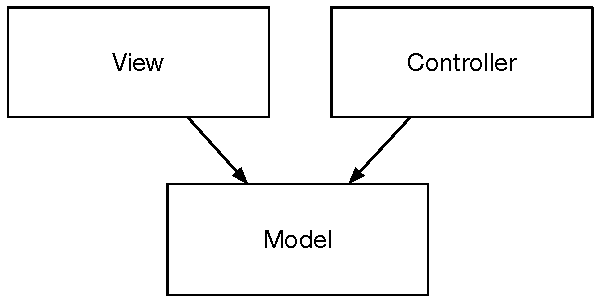
\includegraphics[height=6cm,keepaspectratio]{assets/concept/mvc_1.pdf}
    \caption{Classic MVC}
    \label{fig:mvc_1}
\end{figure}

\subsection{Modern MVC}

Modern MVC has evolved from being a software design pattern which handles components of an application to an architectural design pattern that defines the structure of an application itself. It has many similarities to the Layer Architecture. The responsibilities of each layer are slightly different to the typical presentation, business, and persistence layer definitions.

Most modern web frameworks such as Ruby on Rails, Symfony or the IOS environment refer to themselves as MVC based frameworks. The modern MVC concept has changed slightly. The component definitions are the same, but some responsibilities have shifted. Modern MVC strictly separates the model from the view. All modern frameworks state that the view should have as little logic as possible. Any logic implemented in the view should only be relevant to presentation. The view components should not directly reference the model components\cite{apple_MVC}\cite{symfony_MVC}.

\begin{figure}[H]
    \centering
    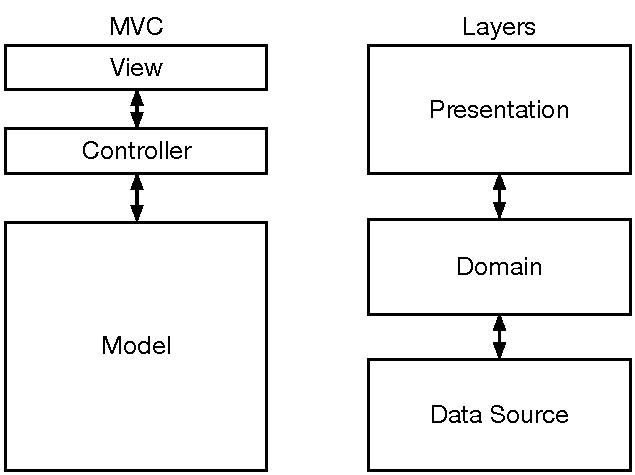
\includegraphics[height=6cm,keepaspectratio]{assets/concept/mvc_2.pdf}
    \caption{Modern MVC vs 3-Tier Layered Architecture}
    \label{fig:mvc_2}
\end{figure}

This division of responsibility has the added benefit of increased testability. GUIs are difficult to test, by removing as much logic as possible from the user interface there is less necessity to test it. The controller and model components can more easily be tested in isolation using normal unit tests\cite{mvp_testing}.

\subsection{MVC Derivatives}

Many MVC derivatives exist. The main differences are where the division of responsibility is made and how it is labeled. MVVM defines a view model instead of a controller. The view model acts as a facade around the model and introduces a data binder element that is responsible for keeping the view and view model synchronised. The MVT, calls the view a template and the controller a view. The slight difference is that the template is basically a static file, with no logic, and placeholders for the data. The Django web framework uses this model, but there is little difference to the other MVC derivatives such as MVP ( model view presenter ). The AngularJS web framework attempts to end the discussion of which design to follow by labelling itself a MVW ( Model View Whatever ) framework\cite{mvw}.


\begin{figure}[H]
    \centering
    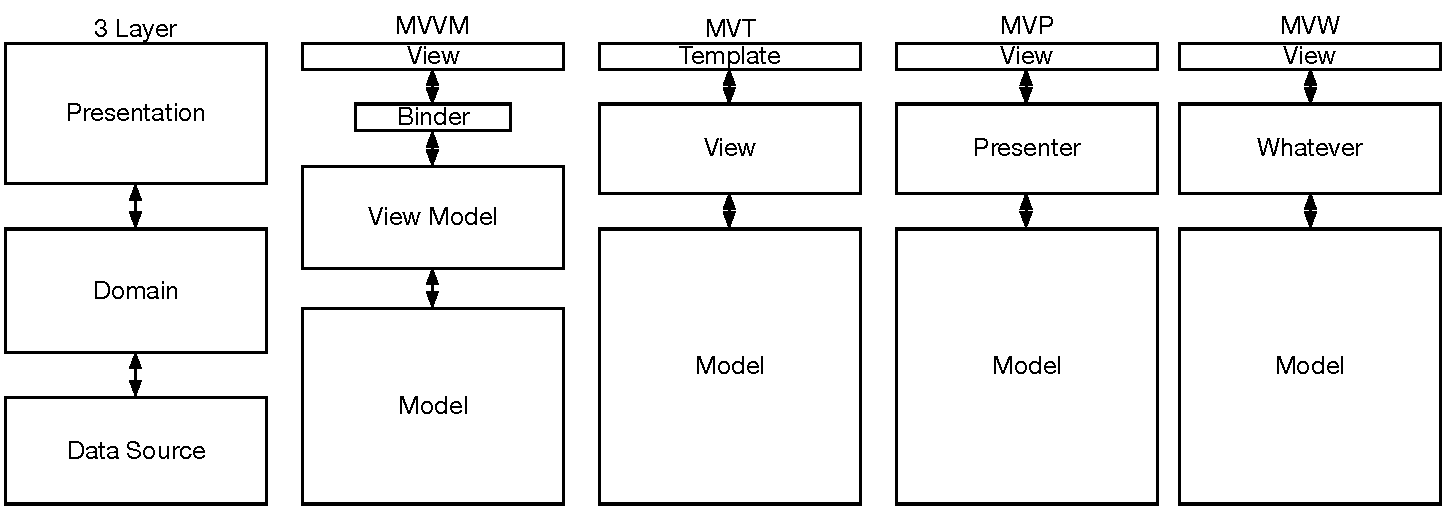
\includegraphics[height=6cm,keepaspectratio]{assets/concept/mvc_3.pdf}
    \caption{MVC Derivatives in relation to 3-Tier Layer}
    \label{fig:mvc_alt}
\end{figure}

\subsection{MVC and Smart Phone Applications}

Although most frameworks and environments targeted toward mobile application development use concepts from MVC, it can be difficult to define strict devision of responsibility, especially in conjunction with services provided from an online server. Often the responsibilities of the controller are reimplemented server side, some model management might occur in the app. Server and application code are developed using different languages and often most likely different developers. One solution is is to develop the app as a thin client, where it basically becomes the view component of MVC and the controllers and model are implemented on the server. Taken to the extreme, the app runs in a standard web browser and server provides the view components that emulate a native mobile user interface. This is referred to as a web app. Any logic in the view is implemented using javascript. Hardware support is limited to what the mobile browser provides access to. In order to extend hardware support a hybrid approach can be used in which the app implements a custom browser view which is extended with native capabilities. Here the division of responsibilities as defined by MVC become fuzzy. A fully native app working in conjunction with a web server will not conform well to the definitions of MVC.

\subsection{Considerations}

From the prioritised requirements defined above two important issues have an impact on architectural design decisions. Cross platform integration and extendability. The image processing and risk assessment algorithms are a complex combination of existing python based libraries and custom code. The rational behind choosing python as the basis is explained in detail in previous chapters. The disadvantage of choosing python for the basis of a mobile application is that is it not easily deployable on mobile hardware. Regardless of the decision to use python, the complexity of these algorithms would make it difficult and costly to implement in a cross platform manner in any language.

The solution is to offload the image processing and risk assessment algorithms to an online server running a python environment. The mobile application can interface with the online server in such a way that the process is transparent to the user.

The requirement for extendability and maintenance ( updatability ) becomes much easier as well. Updating the complex algorithms in multiple languages on multiple platforms and deploying updates to all existing users via the iTunes and Android shop platforms is not necessary. Instead only the server code needs to be updated. In the best case the phone-side app will not have to be updated at all.

Still the question remains, what architecture design pattern best covers the requirements of a mobile app with online server integration.

\subsection{VIPER}

VIPER is a new software architecture pattern which extends MVC with some addition concepts that make it more adaptable to mobile applications, especially when they are extended with online server based services. The classic controller is split into a presenter and a controller, the model component is split into a central data manager communicating with many services and entities\cite{viper}.

\begin{figure}[H]
    \centering
    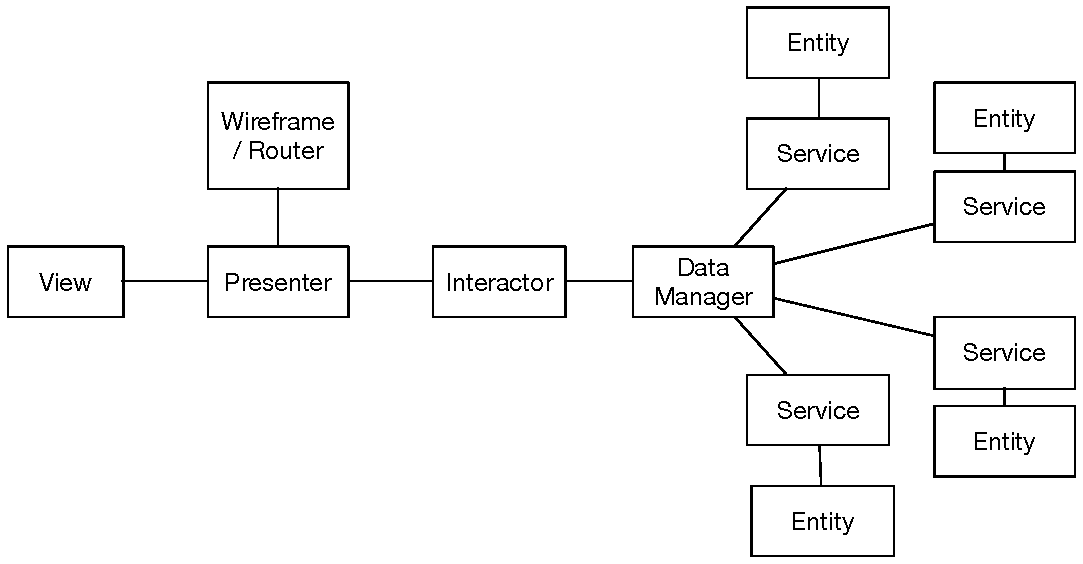
\includegraphics[height=7cm,keepaspectratio]{assets/concept/viper.pdf}
    \caption{VIPER Overview}
    \label{fig:viper}
\end{figure}

\begin{itemize}[label={}]

\item \textbf{View}: The view corresponds to the view as defined in modern MVC definitions, it is a slim component with as little logic as possible. It presents the current state of the models and provides “widgets” with which the user can interact.
\item \textbf{Presenter}: The presenter passes data to the view and handles events from the view. The presenter might perform some basic validation, in the case of a user sign-up scenario, for example, the presenter might validate that a user’s email is indeed formatted as a correct email, it will not validate if the email has already been used by someone else.

\item \textbf{Interactor}: Business logic is handled by the interactor. Most a what the model component in MVC was responsible for is handled here. The interactor however does not know anything about data storage, databases, or persistence. It does not know if data is local or accessible via a network.

\item \textbf{Data Manager}: To the Interactor the data manager looks like a database, with the difference that the it knows how to notify the interactor when data is available. The data manager will receive requests from the interactor, check it’s local cache, perform external service requests if necessary, then pass data back to the interactor once available.
\item \textbf{Service}: Services are encapsulated processes that can be online or local. The service knows how to fetch or store data, it might be a local sqlite database, or it can encapsulate the communication to an online database via a REST-API.

\item \textbf{Entity}: The representation of the actual data. As the entity get passed through the system it might be in the form of a database entry, a json object, or data object.

\item \textbf{Wireframe / Router}: The wireframe initialises all the other classes and handles the transitions to other views in the app. The wireframe handles the current “state” of the app and might implement a “history” allowing the user to transition back to a previous view with the associated other components and data.


\end{itemize}

\section{Mobile Development Strategies}
\subsection{Pure Native vs Hybrid Native vs Hybrid vs Web Apps}

The mobile app market is segmented into several platforms. Each platform has it’s own framework, API, and language specifications and requirements. Android apps are written in java and access the Android APIs, iOS apps in Objective-C or Swift and interface with the iOS frameworks. Android and iOS cover about 94\% of the worldwide mobile market \cite{mobile_market}. A developer must decide which platforms are priorities, and how might programming effort be consolidated across multiple platforms. Several strategies exist, and there are many tool kits and frameworks that can help accelerate development.

\begin{itemize}[label={}]

\item \textbf{Web Apps}: The simplest development strategy is to develop an HTML based web page that is disguised to appear and behave like a mobile app. The web app runs in a normal browser, is deployed from a standard web server. Model mobile web browsers offer javascript APIs that can access various other hardware components of the smart phone such as the compass, GPS/geolocation services, accelerometer, and the camera. Other services will remain inaccessible.

\item \textbf{Hybrid}: A similar strategy is to develop using javascript and html, but to package these elements into a “hollow” native app that is little else than a native view component with an embedded web browser. The web browser url is locked to the internal html files and appears to the user as a mobile app. though the user interface might slightly different that a pure native app. The advantage of a hybrid strategy is that the app can be distributed via the standard app stores increasing it’s marketability. It can also be extended with native components that might otherwise not be accessible to to a web app such as internal file storage and native data storage mechanisms.

\item \textbf{Pure Native}: The developer uses the development environment as provided by the phone manufacturer and has full access to all of the native hardware APIs, development kits and tools. The performance and responsiveness of a pure native app is much better compared to web and hybrid solutions. The user interface is built with the standard UI tools allowing a better user experience because the user is presented with familiar UI elements.

\item \textbf{Hybrid Native}: Recently several cross platform application frameworks have emerged that allow the developer to use a single language that can be compiled across several platforms. These frameworks unify the system and hardware APIs from different platforms into a single API. The limiting factor is how widely the unified API covers all the features the MDApp must integrate.

\end{itemize}



\section{Mobile Frameworks}
9 Cross Platform Mobile Frameworks were identified and compared. The 9 Frameworks were  found using the online Mobile Frameworks Comparison Chart. The target platforms where Android and iOS. The hardware features selected were Camera, Capture, Connection, File and Storage. In addition the framework should include UI Widgets and a free License. The following 9 frameworks were listed:

\begin{itemize}[label={}]
\item \textbf{AppGyver:} AppGyver is a hybrid solution based on Cordova/Phonegap. Cordova/Phonegap apps are programmed in javascript, using standard html/css for the interface, and wrapped in an application that is little more that a full screen web browser. Native functionality is made available through plugins. The AppGyver Supersonic device API does not allow a camera preview to be integrated into the UI or the app, this must be implemented using a 3rd party cordova plugin. The AppGyver Supersonic UI can be used to implement the UI Components of the app, or another UI Framework such as ionic could be integrated. In fact the only difference from AppGyver and ionic is that many AppGyver feature utilises an online developer environment which is a commercial service.

\item \textbf{Application Craft:} Like AppGyver, Application Craft is a based on Cordova/Phonegap. But the developer environment and deployment process is totally bound to the commercial online service. It is not clear from the developer documentation whether the applications are extendable with 3rd party plugins.

\item \textbf{Corona:} Cross-platform native solution, targeted toward game development. C++ and Lua are used for programming. The UI features are game oriented and do not offer many advantages for general mobile apps development.

\item \textbf{Framework7:} This is a professional looking cordova based solution. The UI features are excellent. Native functionality is extendable through 3rd party cordova plugins. Unfortunately Android is only partially supported.

\item \textbf{Gideros:} Gideros is a cross platform native solution that uses Lua for programming targeted toward game development. The feature set is similar to Corona. So are the limitations. The UI is not appropriate to general app development. The developer documentation is not clear regarding camera integration.

\item \textbf{ionic:} ionic is a mature UI framework built on Cordova/Phonegap. ionic is implemented using angular.js and offers a rich set of template directives which can be used to customise the user interface easily. Two-way data binding between logic controllers and view templates is also enabled through angular. The ionic developer also provides an online service that assists in development and deployment. Use of the service is completely optional though.

\item \textbf{Kivy:} Kivy is a python based framework that is compiled to native code. Unfortunately the UI components are not targeted toward general app development and are more game oriented.

\item \textbf{The-M-Project:} This is a hybrid cross platform framework that uses web technologies to provide the UI and logic. It leverages backbone.js to make UI development simpler. Its not clear in the documentation how camera access is enabled and to what extent. The framework does not appear to be based on Cordova/Phonegap so those 3rd part plugins might not be available.

\item \textbf{ViziApps:} Similar to AppGyper and Application Craft. This framework is Cordova/Phonegap based with a strong dependency on a commercial online development and deployment environment.

\end{itemize}

\subsection{Comparison}

\begin{itemize}[label={}]
\item \textbf{Cross-platform Support:} A minimum requirement for cross-platform support is that the framework allows the application to run on iOS and Android devices without any addition configuration.

Enabler of: OE-1, POR-1

\item \textbf{Integrated Camera Access:} The framework allows integrated access to the devices camera APIs. The MDApp will not simply pass the Smartphone User to the native camera mode. Instead the camera preview will be integrated in the MDApp user interface. If available on the native device the MDApp should also be able to set the focal range, center the focal point and be notified via a callback when the camera lens has focused so that it can notify the Smartphone User that it is ready to capture an image.

Enabler of: Image.Capture.Preview, Image.Capture.Trigger, SI-1.*

\item \textbf{Network Connectivity:} The framework allows the MDApp to connect via the internet to the online services required to perform the border analysis and risk assessment calculations. This includes uploading and downloading image files as well as posting and receiving data from an online API.

Enabler of: CI-1.*, CI-2.*, Border.Extract.Calculate, Risk.Assessment.Calculate

\item \textbf{Native File Access:} The framework allows the MDApp to save image files, captured by the camera or downloaded from the border extraction service, to be save internally on the native file system. Image files shall not only be saved in the devices image library but within the MDApp’s allocated storage. On iOS the image files shall be saved in the app internal “/Directory” folder. This directory is accessible and manageable by the user, it is also backed up via the iOS native backup strategies that the Smartphone User would be familiar with. On Android image files and data should be saved on the shared “External Storage” directory. This ensures that files and data are both accessible, backup-able, and persisted in the case of a software update.

Enabler of: SI-2, INT-1, INT-2, INT-3

\item \textbf{Native DB Storage:} Hybrid Apps generally live in a browser based context. Persistence of data is an issue therefore because in browsers data is generally transient. The framework chosen needs to offer a data solution either be tying in to native system data solutions ( CoreData on iOS for example ) or by providing an Sqlite file based solution.

Enabler of: INT-1, INT-2, INT-3, Metadata.Location.*, Metadata.Text.*, Archive.Save, Archive.Browse, Archive.Select.*

\item \textbf{UI Components:} The framework should include graphical user interface components and layout tools that assist in building a user interface that emulates the native look and feel of the platform. At the same time is should be consistent across all platforms. These are two conflicting requirements so some compromise is necessary to balance these aspects.

Enabler of: UI-5, UI-6, POR-1

\item \textbf{Unrestrictive License:} The framework should not be prohibitive with respect to intellectual property or financial cost. It should be open source with no restrictions on the distribution model for the app. The financial cost should be low, or free.

\item \textbf{Unrestrictive License:} Some frameworks are integrated with a service (usually commercial) that allow or restrict development to an online web based development environment. The chosen framework should not restrict development or deployment in any way.


\item \textbf{Advanced MVC Integration:} Does the framework offer tools that assist the developer to adhere to a modern MVC architecture? Integrated data-binding functionality, for example, allows data synchronisation between the view and controller.

Enabler of: TES-1, MOD-1

\end{itemize}

Figure \ref{fig:comp_fw} shows the comparison matrix applied to the 9 mobile cross-platform development framework.

\begin{figure}[H]
    \centering
    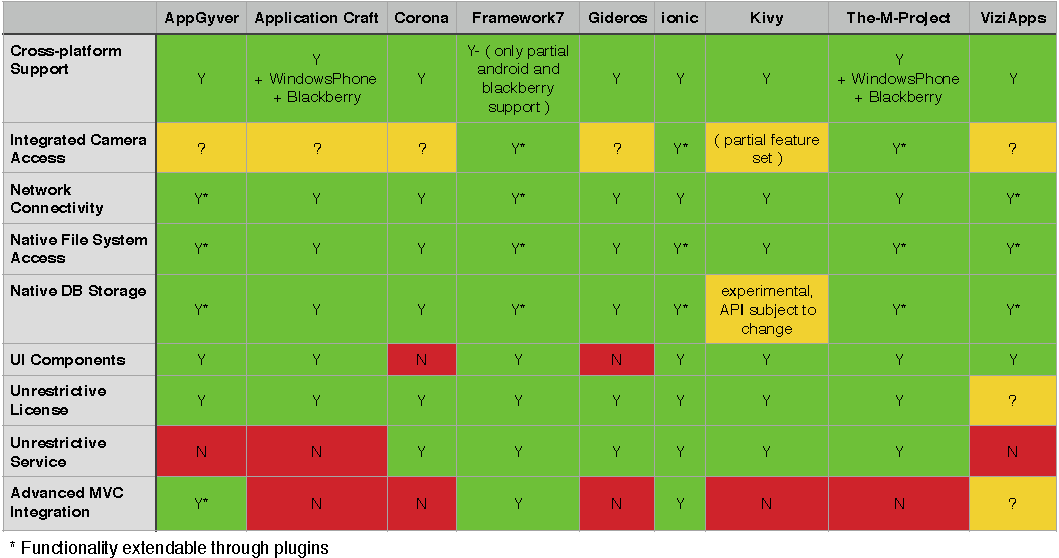
\includegraphics[width=\textwidth,keepaspectratio]{assets/architecture/framework_comparison.pdf}
    \caption{Mobile cross platform frameworks comparison}
    \label{fig:comp_fw}
\end{figure}

Framework7 and ionic score the best in the comparison chart above. Framework7 is a newer framework with no external dependencies. Ionic has been around longer and is basically a mobile UI framework that is built upon AngularJS, bringing with it all the features that make browser based development easier. Two-way data binding, tempting, and RESTful programming resources are some of the highlights of Angular. Because of these features and the widely available programming resources, references, and documentation ionic has been chosen as the framework to implement the MDApp.



\section{Application Structure}
\subsection{Components}

Figure \ref{fig:comp_dia} shows a high level view of the logical layout of the components in the MDApp.

\begin{figure}[H]
    \centering
    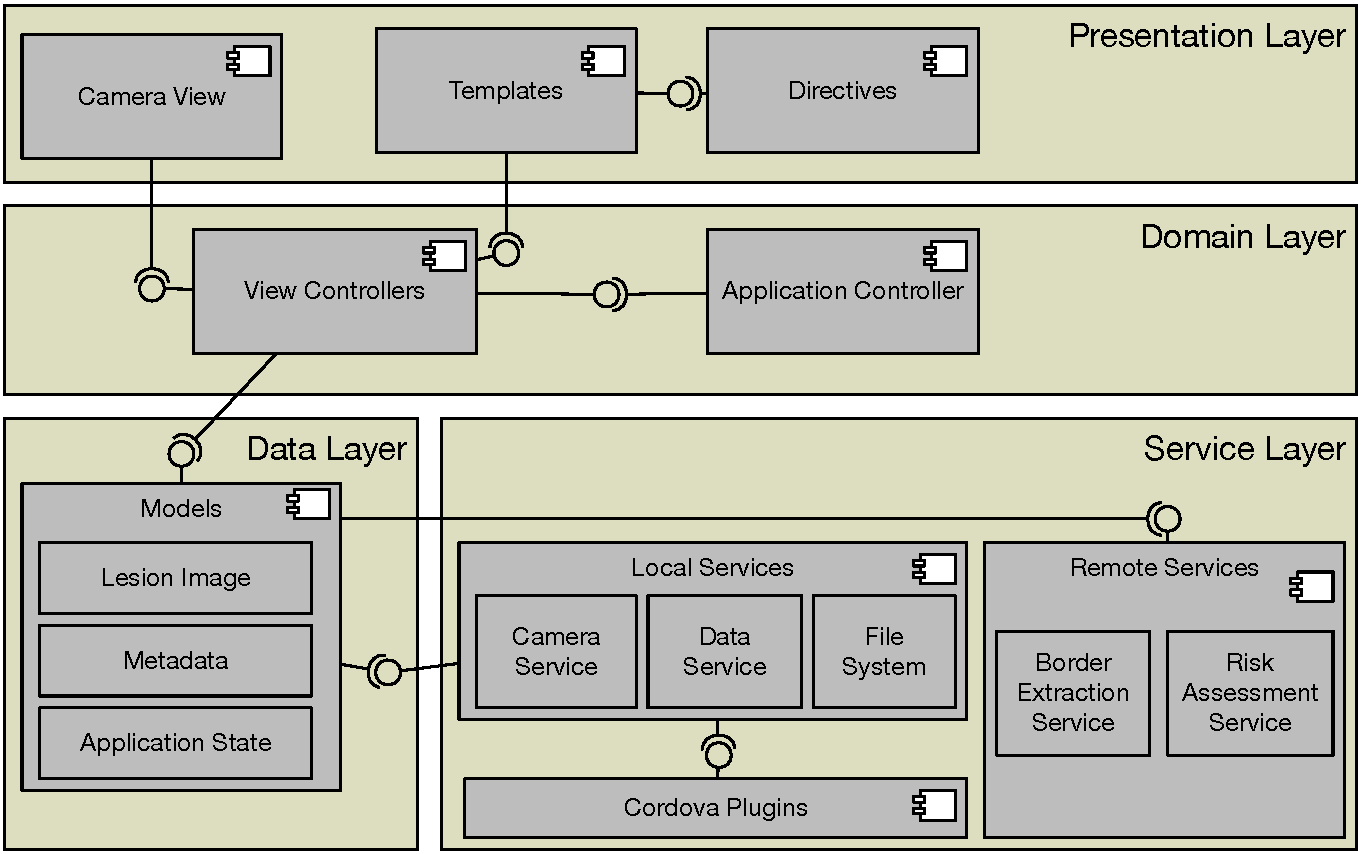
\includegraphics[width=\textwidth,keepaspectratio]{assets/architecture/compontent_diagram.pdf}
    \caption{Component diagram of the MDApp}
    \label{fig:comp_dia}
\end{figure}

\subsubsection{View Controllers}

Each view controller class is responsible for a specific view or partial view of the MDApp. In larger applications there might be multiple view controllers per “page” in a nested hierarchy. The MDApp will only require one controller per page, these are the HomeController, CameraController, AnalysisController and the ArchiveController. Each controller is responsible for preparing the data that will be displayed in the view as well as capturing and processing user events.

\subsubsection{Application Controller}
The application controller is a global controller that can manage the state of the app. It makes sure that the state is persevered when the MDApp is closed and restarted. It can also switch the user automatically from one view to another when appropriate or enable or disable the user interface when some activity is in progress.

\subsubsection{Templates, Directives and Camera View}
Except for the the Camera View all of the pages are created from HTML files that have prepared placeholders called directives. Directives are special markers in the HTML that the Angular framework uses to inject data and specific behaviour into the HTML element. Directives bundle together often used patterns into easily configurable markers that can be embedded into an HTML file.

The Camera View is an exception in the MDApp. The CameraView is an HTML template that overlays a realtime preview of the camera’s input. The realtime preview is not part of the Cordova/Phonegap browser view, it is a platform native view element that is provided by a 3rd party plugin. The cordova-plugin-camera-preview is a crossplatofrm wrapper around native code that allows the browser based javascript to communicate and control the camera preview view.

\subsubsection{Models}
The Models are relatively simple data classes. The MDApp does not require much buisiness logic for the data. The Models encapsulate some communication with some of the services so that the controllers can remain as simple as possible.

\subsubsection{Local Services}
The local services classes are just wrappers around the Cordova plugins. Cordova plugins offer a "raw" javascript api, the service classes will hide some of the complexity by making only the relevant functions available to the MDApp.

\subsubsection{Remote Services}
The remote services leverage the angular \$resource factory which provides easily configurable RESTful communication to online servers.

\subsubsection{Cordova Plugins}

In a hybrid architecture most of the logic is programmed in javascript, just like a normal web page. Communication with native system components and hardware APIs that a normal browser based environment does not have access can be enabled through plugins. Ideally these plugins unify the native APIs across all platforms. The MDApp uses the following cordova plugins:

   \paragraph{cordova-plugin-camera-preview}
   \paragraph{cordova-plugin-file-transfer}
   \paragraph{Cordova-sqlite-storage}

\subsection{Classes}

The class diagram in figure \ref{fig:class_dia} shows the structure and connections between the main classes of the MDApp. The service layer classes are singletons that encapsulate the functionality of some plugin into an easy to manage form. Static class level methods and attributes are underlined. The other methods and attributes have object level scope.

\begin{figure}[H]
    \centering
    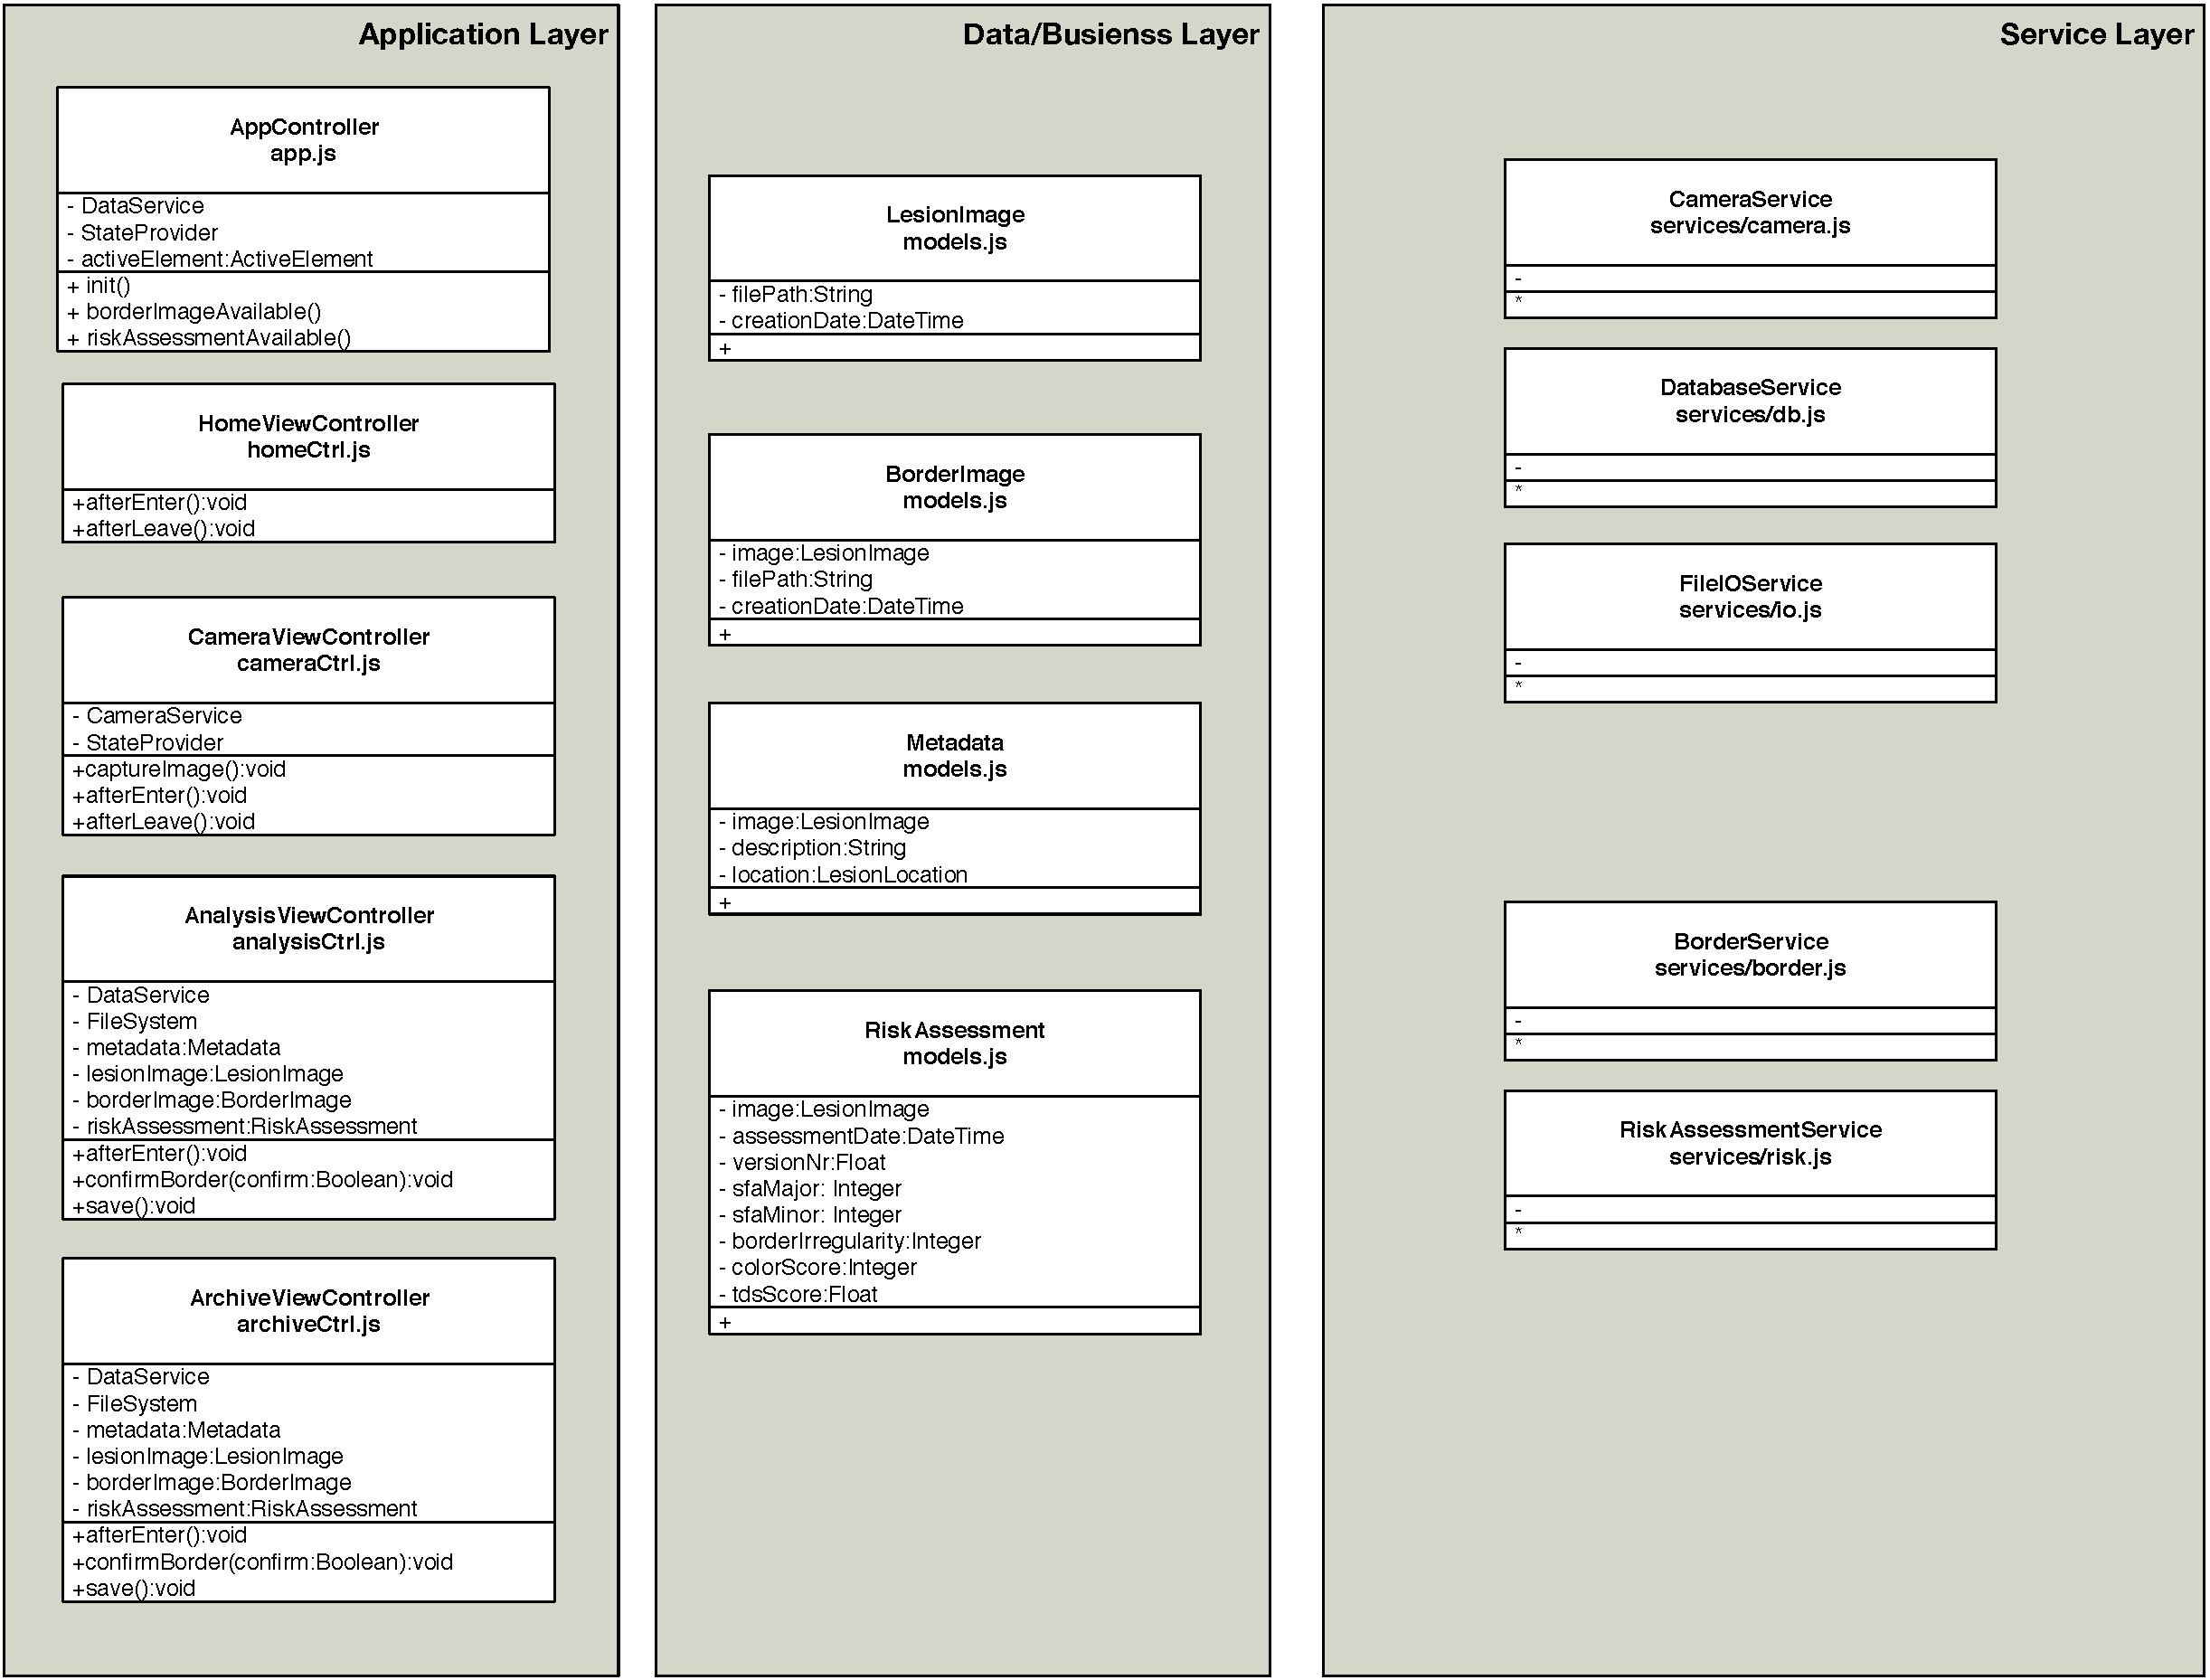
\includegraphics[width=\textwidth,keepaspectratio]{assets/architecture/class_diagram.pdf}
    \caption{Component diagram of the MDApp}
    \label{fig:class_dia}
\end{figure}

    \subsubsection{Application Layer}
        \paragraph{AppController}
                            \begin{longtable}[H]{  | >{\bfseries}l | l | l | l | l | }

                    \hline

                    Name
                    & \multicolumn{4}{l |}{AppController} \\ \hline

                    Description
                    & \multicolumn{4}{p{8.5cm} |}{The AppController manages the global state of the app. It can disable UI elements when the app needs to wait for longer processes. It can restore the previous state of the app after it has been reopened or updated.} \\ \hline

                    Type
                    & \multicolumn{4}{l |}{Class}
                    \\ \hline

                    Implemented In
                    & \multicolumn{4}{l |}{app.js}
                    \\ \hline

                    Attributes
                    & Name & Type & \multicolumn{2}{p{6.5cm} |}{Description} \\ \hline
                        & \$state & class & \multicolumn{2}{p{6.5cm} |}{
                        The \$state object is provided by the angular ui-router and is used to define pages in the app. It can be used to query or set the ui state. The AppController uses the \$state to automatically move the user from the camera view to the analysis view when the border data has become available, for example.
                        } \\ \hline
                        & MDAppState & class & \multicolumn{2}{p{6.5cm} |}{
                        The MDAppState stores data the the AppController might need to restore it's state after a restart.
                        } \\ \hline
                        & uiDisabled & boolean & \multicolumn{2}{p{6.5cm} |}{
                        This variable is used to trigger changes in the ui. Through 2-way binding the ui components in the view will become disabled or enabled respectivly.
                        } \\ \hline
                        & tabStates & object & \multicolumn{2}{p{6.5cm} |}{
                        This javascript object stored the disabled-state of the individual tab components in the ui. The AppController disabiles or enables specific tab elements based on the state of the app and the data currently available.
                        } \\ \hline


                    Methods
                    & Name & Parameter & Return Type & Description \\ \hline

                        &


                \end{longtable}




\section{User Interface}
    
        \subsubsection{Logical Data Model}

            \begin{figure}[H]
                \centering
                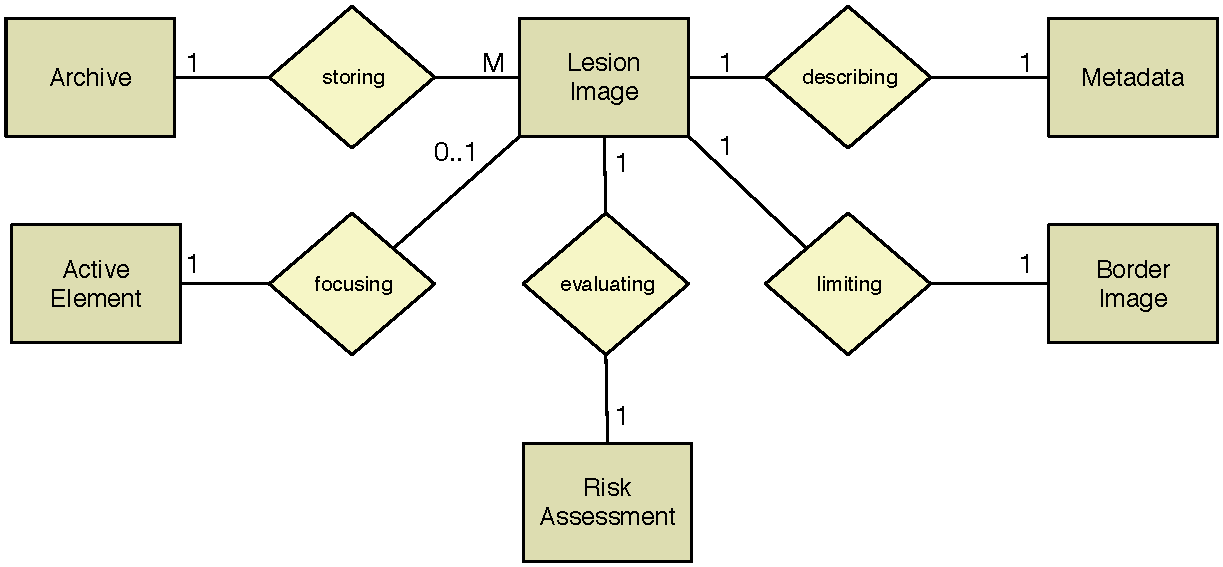
\includegraphics[width=\textwidth]{assets/requirements/EntRel.pdf}
                \caption{Patial data model of the Melanoma Detection App}
                \label{fig:partial_data_model}
            \end{figure}


        \subsubsection{Data Dictionary}

                \begin{longtable}[H]{ | l | p{3.0cm} | p{2.5cm} | p{1.0cm} | p{2.5cm} | }

                    \hline
                    \textbf{Data element} & \textbf{Description} & \textbf{Componsition or data type} & \textbf{Length} & \textbf{Values} \\ \hline

                    \hypertarget{lesion_image}{Lesion Image} & reference to the captured image &

                        \specialcell[t]{Image ID
                           \\ + File Path
                           \\ + Creation Date
                        }

                     & & \\ \hline

                    Image ID & unique identifier for an image &
                    integer & 11 & system-generated sequential integer beginning with 1 \\ \hline

                    File Path & location of a file on the file system &
                    string & 256 &  \\ \hline

                    Creation Date & date and time that a file was created &
                    DDMMYYYYHHSS &  &  \\ \hline

                    Metadata & information describing the lesion and it's location &

                        \specialcell[t]{\hyperlink{lesion_image}{Lesion Image}
                           \\ + Lesion Description
                           \\ + Lesion Location
                        }

                     & & \\ \hline

                    Lesion Description & User defined text that describes the lesion &
                    alphanumeric &  &  \\ \hline

                    Lesion Location & information describing the lesion location on the body &

                        \specialcell[t]{\hyperlink{lesion_image}{Lesion Image}
                           \\ + Body Location ID
                           \\ + X Coordinate
                           \\ + Y Coordinate
                        }

                     & & \\ \hline


                    Body Location ID & id of a region on the body &
                    integer & 2 & TBD \\ \hline

                    X Coordinate & x coordinate of the lesion in the region specified by the body location id &
                    integer & 128 &  \\ \hline

                    Y Coordinate & y coordinate of the lesion in the region specified by the body location id &
                    integer & 128 &  \\ \hline

                    Border Image & data that defines the outline of the lesion area &

                        \specialcell[t]{\hyperlink{lesion_image}{Lesion Image}
                           \\ + File Path
                           \\ + Creation Date
                        }

                     & & \\ \hline

                    Risk Assessment &  &

                        \specialcell[t]{\hyperlink{lesion_image}{Lesion Image}
                            \\ + Assessment Date
                            \\ + Version Number
                            \\ + SFA Major
                            \\ + SFA Minor
                            \\ + Border Irregularity
                            \\ + Color Score
                            \\ + \hyperlink{tds_score}{TDS Score}
                        }

                    & & \\ \hline

                    Assessment Date & date and time that the risk assessment was calculated &
                    DDMMYYYYHHSS &  &  \\ \hline

                    Version Number & version number of the risk assessment service software &
                    integer & 4 &  \\ \hline

                    SFA Major & measure of symmetry of the lesions major axis &
                    integer & 3 & 0 - 360 \\ \hline

                    SFA Minor & measure of symmetry of the lesions minor axis &
                    integer & 3 & 0 - 360 \\ \hline

                    Border Irregularity & measure of irregulatiry of the lesion's border &
                    integer & 1 & 0 - 8 \\ \hline

                    Color Score & number of specific colors found in the lesion's image &
                    integer & 1 & 0 - 8 \\ \hline

                    \hypertarget{tds_score}{TDS Score} & weighted linear combination of the image features summarizing the risk assessment  &
                    float &  & 1 - 8.9 \\ \hline

                    Archive &  &

                        \specialcell[t]{Archive ID
                            \\ + \hyperlink{lesion_image}{Lesion Image}
                            \\ + Metadata
                            \\ + Border
                            \\ + Risk Assessment
                            \\ + Archive Date
                        }

                     & & \\ \hline


                    Color Score & number of specific colors found in the lesion's image &
                    integer & 1 & 0 - 8 \\ \hline

                \end{longtable}


        \subsubsection{Data analysis}
            \paragraph{CRUD Matrix}

                \begin{figure}[H]
                    \centering
                    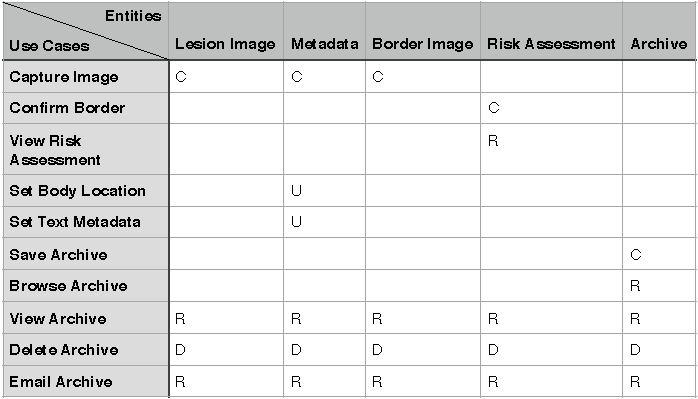
\includegraphics[width=\textwidth]{assets/requirements/CRUD.pdf}
                    \caption{CRUD matrix for Melanoma Detection App}
                    \label{fig:crud}
                \end{figure}

        \subsubsection{Reports}
            \paragraph{Email Report}
                When the Smartphone User chooses to send an archive as an email, the data must be flattened into a format that is email compatible. The body of the email will be an html formated document that displays the lesion image, the calculated border, the risk assessment data and the associated metadata.






\chapter{Testing}
\section{Section Title}

\chapter{Application Implementation}
\subsection{Section Title}

\chapter{Conclusions}
The goals of this project have mostly been completed. Some topics were more complex than originally estimated and some compromises were made regarding the details of each topic. This project can be regarded as a high level overview of the components necessary to build a smart phone based melanoma detection application. Several topics could probably become the basis of further dedicated projects and expanded on. Each goal is reviewed in more detail below.

\noindent
\begin{itemize}
\item[1] The current state of the available medical mobile apps was explored. The apps were grouped into categories and compared. While the overall majority of apps were providing an educational service, many diagnostic apps were identified. In comparison with other research from 2013 it could be shown that the availability of apps that provide a diagnostic function is increasing.

\item[2] A large part of the effort that went into this project was dedicated to researching and becoming familiar with image processing and analysis algorithms. During the exploration and experimentation of methods to automatically identify the skin lesion some novel insights were gained.

\item[3] Much research exists regarding automatic risk assessment of melanoma in images captured with a dermatoscope, less so for images captured with a smart phone camera. The difficulty this introduces became apparent. It remains unclear after this project how much the methods for dermatoscopic image risk assessment are actually applicable to images captured with a smart phone.

\item[4] One of the stated goals was to choose a specific algorithm and data with which to proceed. The choice of algorithm became limited by the time available for research and prototyping. Basically what worked in the experimentation phase was chosen. The time it would have taken to implement and compare several algorithms was not available.

\item[5] Putting the research together into a working algorithm was not difficult as far as programming was concerned. The python based prototypes form the experimentation phase could be reused easily in the final algorithm. The most effort was spent in actually reviewing results and trying to achieve and overview of how well the different components actually worked on all the sample image sets. A lot of development time went into building tools that accelerated the review and comparison effort. Even with the tools though it was not possible to do much comparing and optimisation because the review process still took several days to complete. So, although an algorithm was implemented that could identify and assess a skin lesion image, it’s performance has not been adequately reviewed and optimised.

\item[6] A concept was created for a mobile medical app that would provide the user with a risk assessment based on the algorithms implemented. The amount of effort required for this was initially underestimated due to an unfamiliarity with requirements engineering principals. After several iterations and time spent learning the concepts a relatively complete concept was created. It became clear that requirements engineering is not a static process but requires several iterations where insights gained in later steps must flow back into the requirements definitions. This will be a valuable takeaway from this project.

\item[7] A proof of concept app was developed in tandem with the requirements engineering process. The proof of concept evolved from a static mockup into an actual app and was used to evaluated and refine the requirement definitions. Although the proof of concept itself is not described in this document, the concepts described in the requirements and design chapters flow from the evolution of the prototype.

\end{itemize}





\bibliography{references}{}
\bibliographystyle{plain}

\chapter{Appendix}
\section{Optimizations}

\subsection{Border Extraction}

\subsection{SFA Threshold}



\end{document}